% Evidentirane korisnikove podele s002/s009/s015/s023/s024/s032/s048/s049: 54 originala, 62 okvira.
\documentclass[aspectratio=169,11pt]{beamer}
\newcommand{\ETFTemaPutanja}{../_zajednicko/etf-v1}
\makeatletter
\edef\input@path{{\ETFTemaPutanja/}}
\makeatother
\usepackage{stil,dijagrami}
% Lokalna primena pravila odobrenih u 01; zamrznuta tema etf-v1 se ne menja.
\definecolor{DEisticanje}{HTML}{A32638}
\colorlet{DEcrvena}{DEisticanje}
\setbeamercolor{alerted text}{fg=DEisticanje}
\tikzset{DEstrelica/.style={wire,-{Latex[length=2mm]}}}
\renewcommand{\Oznaka}[1]{\par{\fontsize{10}{12}\selectfont\color{Muted}#1\par}}
\setlength{\parskip}{2pt}
\title[Digitalna elektronika 1 · 2021/22]{Sinteza kombinacionih mreža}
\author{prof. dr Lazar Saranovac}
\institute{Katedra za elektroniku, Elektrotehnički fakultet}
\date{2021/22}
\begin{document}
% Original: PDF strana 1, gornji slajd.
\slajdid{02-s001}
\begin{frame}[label=02-s001]
\centering
\vfill
% element: 02-s001:e01
{\fontsize{28}{33}\selectfont\color{DEplava}Sinteza\\[4mm]kombinacionih mreža}\par
\par\vspace{8mm}
{\large Digitalna elektronika 1}\par
\par\vspace{2mm}
{\normalsize prof. dr Lazar Saranovac · 2021/22}
\vfill
\end{frame}

\slajdid{02-s002}
\begin{frame}[label=02-s002]{Šta znači „trenutno“ stanje ulaza?}
\fontsize{11}{12.5}\selectfont
% element: 02-s002:e01
Kombinacione mreže su digitalni sistemi kod kojih izlazi zavise samo od stanja ulaza. \alert{???}
\par\vspace{1.5mm}
Od kojih stanja ulaza? Jučerašnjih? Od onih pre 100 ms? Bivših, sadašnjih, budućih?\par
\textbf{Moramo dodati vremensku odrednicu!}
\par\vspace{1.5mm}
\Rezultat{Kombinacione mreže su digitalni sistemi kod kojih izlazi zavise samo od \alert{trenutnog} stanja ulaza.}
\par\vspace{1.5mm}
% element: 02-s002:e02
\textbf{Trenutnog?} Pojam koji često koristimo ne ulazeći dublje u njegovo značenje.\par
Ako su se ulazi promenili u nekom trenutku vremena, da li su se i izlazi \alert{trenutno} promenili?
\par\vspace{1.5mm}
Kada kažemo da se nešto trenutno dešava, obično podrazumevamo vremenske margine: u realnom fizičkom svetu promena se ne dešava u beskonačno kratkom vremenskom intervalu.
\end{frame}

\slajdid{02-s002b}
\begin{frame}[label=02-s002b]{Promena ulaza i kašnjenje logičkog kola}
% element: 02-s002b:e01
Šta može da se desi u digitalnom sistemu realizovanom kao kombinaciona mreža?
\par\vspace{4mm}
% element: 02-s002b:e02
\Rezultat{Kada se promene ulazi, izlazi se \alert{ne menjaju odmah}. Postoji vremenski interval u kome tvrdnja o trenutnom stanju ne važi: \alert{stanja izlaza nisu poznata}.}
\par\vspace{4mm}
% element: 02-s002b:e03
\textbf{Zašto?}\par\vspace{2mm}
Logička kola ne mogu trenutno da reaguju na promenu ulaznih promenljivih: njihov odziv ograničavaju fizički procesi. Izlazi će se promeniti tek posle nekog vremena.
\par\vspace{4mm}
\Rezultat{\alert{Kašnjenje logičkog kola.}}
\end{frame}

% Original: PDF strana 2, gornji slajd.
\slajdid{02-s003}
\begin{frame}[label=02-s003]{Kašnjenje invertora pri promeni signala}
% element: 02-s003:e01
\begin{columns}[c,onlytextwidth]
\begin{column}{.72\textwidth}
Signal je fizička veličina koja nosi informaciju o logičkim nulama i jedinicama.
\end{column}
\begin{column}{.24\textwidth}\centering
\begin{tikzpicture}[DEoznaka]
\node[not gate US,draw,minimum width=8mm,minimum height=7mm] (g) at (0,0) {};
\draw[DEvod] (g.input)--++(-.35,0) node[left] {\(x(t)\)};
\draw[DEvod] (g.output)--++(.35,0) node[right] {\(y(t)\)};
\end{tikzpicture}
\end{column}
\end{columns}
\par\vspace{2mm}
% element: 02-s003:e02
\begin{columns}[T,onlytextwidth]
\begin{column}{.43\textwidth}\centering
\Oznaka{Idealizovani odziv}\vspace{3mm}
\begin{tikzpicture}[DEoznaka,x=10mm,y=6.2mm]
\draw[DEstrelica] (-.7,2.55)--(3.8,2.55) node[below] {\(t\)};
\draw[DEstrelica] (0,2.40)--(0,4.35) node[left] {\(x(t)\)};
\draw[DEstrelica] (-.7,-.1)--(3.8,-.1) node[below] {\(t\)};
\draw[DEstrelica] (0,-.25)--(0,1.7) node[left] {\(y(t)\)};
\node[above left,inner sep=1pt] at (0,3.65) {=1};\node[above left,inner sep=1pt] at (0,2.75) {=0};
\node[above left,inner sep=1pt] at (0,1) {=1};\node[above left,inner sep=1pt] at (0,.1) {=0};
\draw[DEvod] (-.5,2.75)--(.6,2.75)--(.6,3.65)--(1.6,3.65)--(1.6,2.75)--(3.5,2.75);
\draw[DEvod] (-.5,1)--(.6,1)--(.6,.1)--(1.6,.1)--(1.6,1)--(3.5,1);
\draw[dashed] (0,3.65)--(.6,3.65);
\draw[dashed] (.6,2.75)--(.6,-.25) node[below] {\(t_1\)};
\draw[dashed] (1.6,2.75)--(1.6,-.25) node[below] {\(t_2\)};
\draw[DEcrvena] (-.8,-.65)--(3,4.15) (-.8,4.15)--(3.5,-.65);
\end{tikzpicture}

\end{column}
\begin{column}{.53\textwidth}\centering
\Oznaka{Odziv sa kašnjenjem}\vspace{3mm}
\begin{tikzpicture}[DEoznaka,x=8.5mm,y=6.2mm]
\draw[DEstrelica] (-.7,2.55)--(3.8,2.55) node[below] {\(t\)};
\draw[DEstrelica] (0,2.40)--(0,4.35) node[left] {\(x(t)\)};
\draw[DEstrelica] (-.7,-.1)--(3.8,-.1) node[below] {\(t\)};
\draw[DEstrelica] (0,-.25)--(0,1.7) node[left] {\(y(t)\)};
\node[above left,inner sep=1pt] at (0,3.65) {=1};\node[above left,inner sep=1pt] at (0,2.75) {=0};
\node[above left,inner sep=1pt] at (0,1) {=1};\node[above left,inner sep=1pt] at (0,.1) {=0};
\draw[DEvod] (-.5,2.75)--(.6,2.75)--(.6,3.65)--(1.6,3.65)--(1.6,2.75)--(3.5,2.75);
\draw[DEvod] (-.5,1)--(1.15,1)--(1.15,.1)--(2.5,.1)--(2.5,1)--(3.5,1);
\draw[dashed] (0,3.65)--(.6,3.65) (0,.1)--(1.15,.1);
\draw[dashed] (.6,2.75)--(.6,-.3) (1.6,2.75)--(1.6,-.3);
\draw[dashed] (1.15,.1)--(1.15,-.3) (2.5,.1)--(2.5,-.3);
\draw[DEcrvena,<->] (.6,-.25)--(1.15,-.25) node[midway,below] {\(t_{pHL}\)};
\draw[DEcrvena,<->] (1.6,-.25)--(2.5,-.25) node[midway,below] {\(t_{pLH}\)};


\draw[DEcrvena,<->] (.6,4.05)--(1.6,4.05) node[midway,above,inner sep=1pt] {\(T_{\mathrm{ul}}\)};
\draw[DEcrvena,<->] (1.15,1.42)--(2.5,1.42) node[midway,above,inner sep=1pt] {\(T_{\mathrm{izl}}\)};
\node[right,inner sep=1pt,text=DEcrvena] at (4.2,2.0) {\(T_{\mathrm{ul}}=T_{\mathrm{izl}}\;???\)};
\end{tikzpicture}

\end{column}
\end{columns}
\par\vspace{2mm}
% element: 02-s003:e03
\begin{columns}[T,onlytextwidth]
\begin{column}{.47\textwidth}
\(\textcolor{DEcrvena}{t_{pHL}}\): kašnjenje pri prelazu izlaza \(H\to L\).
\end{column}
\begin{column}{.49\textwidth}
\(\textcolor{DEcrvena}{t_{pLH}}\): kašnjenje pri prelazu izlaza \(L\to H\).
\end{column}
\end{columns}
\par\vspace{1mm}
\Oznaka{\(p\) — propagation; \(H\) — high, \(H=1\); \(L\) — low, \(L=0\).}
\end{frame}

\slajdid{02-s004}
\begin{frame}[label=02-s004]{Srednje kašnjenje i kratak impuls}
\setlength{\abovedisplayskip}{4pt}\setlength{\belowdisplayskip}{4pt}
% element: 02-s004:e01
\Rezultat{Zapamtiti: \(\textcolor{DEcrvena}{t_{pHL}\ne t_{pLH}}\).}
\par\vspace{2mm}
\begin{columns}[T,onlytextwidth]
\begin{column}{.67\textwidth}
% element: 02-s004:e02
Srednje kašnjenje logičkog kola:
\[t_p=\frac{t_{pHL}+t_{pLH}}{2}\]
Za pojednostavljen prikaz \alert{nekih} pojava uzimamo
\[t_{pHL}=t_{pLH}=t_p.\]
% element: 02-s004:e04
\textbf{Da li je izlazni signal samo zakašnjena verzija ulaznog?}\par\vspace{1mm}
Može se promeniti oblik i trajanje impulsa, a impuls može i da izostane.\par\vspace{1mm}
\alert{Ishod zavisi od trajanja ulaznog impulsa u odnosu na kašnjenja kola.}
\end{column}
\begin{column}{.29\textwidth}\centering
% element: 02-s004:e03
\Oznaka{Kratak impuls}\par\vspace{3mm}
\begin{tikzpicture}[DEoznaka,x=8.2mm,y=7.5mm]
\draw[DEstrelica] (-.7,2.25)--(3.8,2.25) node[below] {\(t\)};
\draw[DEstrelica] (0,2.10)--(0,4.05) node[left] {\(x(t)\)};
\draw[DEstrelica] (-.7,-.1)--(3.8,-.1) node[below] {\(t\)};
\draw[DEstrelica] (0,-.25)--(0,1.7) node[left] {\(y(t)\)};
\node[above left,inner sep=1pt] at (0,3.35) {=1};\node[above left,inner sep=1pt] at (0,2.45) {=0};
\node[above left,inner sep=1pt] at (0,1) {=1};\node[above left,inner sep=1pt] at (0,.1) {=0};
\draw[DEvod] (-.5,2.45)--(.6,2.45)--(.6,3.35)--(.85,3.35)--(.85,2.45)--(3.5,2.45);
\draw[DEvod] (-.5,1)--(2.8,1)--(2.8,.1)--(3.05,.1)--(3.05,1)--(3.5,1);
\draw[dashed] (.6,3.35)--(.6,-.35) (2.8,.1)--(2.8,-.35) (0,.1)--(2.8,.1);
\draw[DEcrvena,<->] (.6,-.3)--(2.8,-.3) node[midway,below] {\(t_p\)};
\end{tikzpicture}

\end{column}
\end{columns}
\end{frame}

\slajdid{02-s005}
\begin{frame}[label=02-s005]{Maksimalna specificirana kašnjenja}
\begin{columns}[T,onlytextwidth]
\begin{column}{.39\textwidth}\centering
% element: 02-s005:e01
\begin{tikzpicture}[DEoznaka,x=8.6mm,y=8mm]
\draw[DEstrelica] (-.7,2.25)--(3.8,2.25) node[below] {\(t\)};
\draw[DEstrelica] (0,2.10)--(0,4.05) node[left] {\(x(t)\)};
\draw[DEstrelica] (-.7,-.1)--(3.8,-.1) node[below] {\(t\)};
\draw[DEstrelica] (0,-.25)--(0,1.7) node[left] {\(y(t)\)};
\node[above left,inner sep=1pt] at (0,3.35) {=1};\node[above left,inner sep=1pt] at (0,2.45) {=0};
\node[above left,inner sep=1pt] at (0,1) {=1};\node[above left,inner sep=1pt] at (0,.1) {=0};
\draw[DEvod] (-.5,2.45)--(.6,2.45)--(.6,3.35)--(1.6,3.35)--(1.6,2.45)--(3.5,2.45);
\draw[DEvod] (-.5,1)--(1.15,1)--(1.15,.1)--(2.5,.1)--(2.5,1)--(3.5,1);
\fill[DEcrvena!15] (.6,.1) rectangle (1.15,1);
\fill[DEcrvena!15] (1.6,.1) rectangle (2.5,1);
\foreach \a/\b in {.6/1.15,1.6/2.5}{
 \begin{scope}
 \clip (\a,.1) rectangle (\b,1);
 \foreach \x in {0,.12,...,3.5}{\draw[DEcrvena,thin] (\x,.1)--++(.9,.9);}
 \end{scope}
 \draw (\a,.1) rectangle (\b,1);
}
\draw[dashed] (0,3.35)--(.6,3.35) (0,.1)--(.6,.1);
\draw[dashed] (.6,2.45)--(.6,-.3) (1.6,2.45)--(1.6,-.3);
\draw[dashed] (1.15,.1)--(1.15,-.3) (2.5,.1)--(2.5,-.3);
\draw[DEcrvena,<->] (.6,-.25)--(1.15,-.25) node[midway,below] {\(t_{pHL}\)};
\draw[DEcrvena,<->] (1.6,-.25)--(2.5,-.25) node[midway,below] {\(t_{pLH}\)};


\draw[DEcrvena,-{Latex[length=1.6mm]}] (.65,-1.3)--(1.15,-.8);
\draw[DEcrvena,-{Latex[length=1.6mm]}] (3.1,-1.3)--(2.5,-.8);
\node[DEcrvena,below,inner sep=1pt] at (.65,-1.3) {Sigurno 0};
\node[DEcrvena,below,inner sep=1pt] at (3.1,-1.3) {Sigurno 1};
\end{tikzpicture}

\par\vspace{2mm}\Oznaka{Šrafirano: izlaz može biti 0 ili 1.}
\end{column}
\begin{column}{.58\textwidth}
\Rezultat{\alert{Maksimalna} vremena \(t_{pHL}\) i \(t_{pLH}\) određuju kada smo \alert{sigurni} u novo stanje izlaza.}
\par\vspace{2mm}
Promena može nastupiti i ranije; po isteku odgovarajućeg maksimalnog vremena novo stanje je sigurno uspostavljeno.
\par\vspace{2mm}
% element: 02-s005:e02
Stvarno kašnjenje zavisi od napajanja, temperature, starosti i konkretnog primerka kola: \alert{promenljivo je i za isto kolo}.
\par\vspace{2mm}
% element: 02-s005:e03
Proizvođač specificira granice za \alert{tip kola}. One važe za \alert{sve primerke} tog tipa u specificiranim uslovima; stvarna kašnjenja primeraka mogu se razlikovati.
\end{column}
\end{columns}
\end{frame}

% Original: PDF strana 3, donji slajd.
\slajdid{02-s006}
\begin{frame}[label=02-s006]{Kada je izlaz kombinacione mreže važeći?}
% element: 02-s006:e01
\par\Rezultat{Izlaz zavisi od „trenutnih“ ulaza tek \alert{po završetku prelaznih procesa}.}
\par\vspace{5mm}
% element: 02-s006:e02
\begin{enumerate}
\item Promena ulaza se prenosi kroz pojedina logička kola sa kašnjenjem.
\item Vreme do važećeg izlaza zavisi od kašnjenja duž putanja kroz mrežu.
\end{enumerate}
\par\vspace{5mm}
% element: 02-s006:e03
\Oznaka{Neželjeni efekat}\par\vspace{2mm}
U prelaznom intervalu mogu se pojaviti \alert{lažne nule i jedinice} na izlazu.\par\vspace{3mm}
Ovoj pojavi posvetićemo posebnu pažnju pri sintezi kombinacionih mreža.
\end{frame}

% Original: PDF strana 4, gornji slajd.
\slajdid{02-s007}
\begin{frame}[label=02-s007]{Sinteza i kriterijumi minimizacije}
% element: 02-s007:e01
Pod \alert{minimizacijom} se najčešće podrazumeva minimizacija:
\par\vspace{3mm}
\begin{itemize}
\item broja upotrebljenih logičkih kola;
\item ukupnog broja ulaza u logička kola.
\end{itemize}
\par\vspace{5mm}
% element: 02-s007:e02
Može se govoriti i o minimizaciji:
\par\vspace{3mm}
\begin{itemize}
\item broja upotrebljenih \alert{komponenti};
\item ukupnog kašnjenja signala od ulaza do izlaza;
\item drugih zahteva konkretne realizacije.
\end{itemize}
\end{frame}

\slajdid{02-s008}
\begin{frame}[label=02-s008]{Integrisana kola, čip i DIP kućište}
% element: 02-s008:e01
Standardna logička kola dostupna su kao integrisane komponente.\par
\textbf{SSI} (\emph{Small Scale Integration}): do 100 komponenti, odnosno oko 10 gejtova u jednom čipu.\par
Gejt je standardno logičko kolo.
\par\vspace{3mm}
% element: 02-s008:e02
\begin{columns}[T,onlytextwidth]
\begin{column}{.24\textwidth}\centering
\Oznaka{Čip}\par\vspace{3mm}
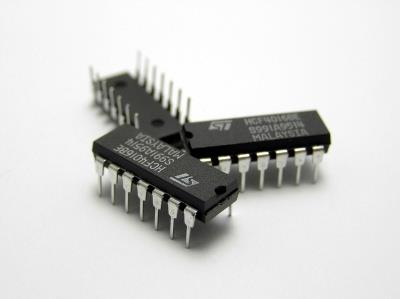
\includegraphics[width=.78\linewidth]{slike/izvorne/s008_integrisana_kola.jpg}
\par\vspace{1mm}
% element: 02-s008:e03
\Oznaka{\(1\,\mathrm{inch}=25{,}4\,\mathrm{mm}\)\\[1mm]
\(1\,\mathrm{mil}=10^{-3}\,\mathrm{inch}\)}
\end{column}
\begin{column}{.37\textwidth}\centering
\Oznaka{Raspored priključaka}\par\vspace{2mm}
\makebox[\linewidth][c]{% Pogled odozgo: četiri dvoulazna I kola u DIP-14 kućištu.
% Svaki vod se završava na odgovarajućem fizičkom pinu; napajanje i masa
% ostaju posebni priključci kućišta, bez prikaza unutrašnjih naponskih vodova.
\begin{tikzpicture}[font=\fontsize{9}{10.5}\selectfont,x=8mm,y=5.5mm,
  DEunutrasnje/.style={and gate US,draw,logic gate inputs=nn,
    minimum width=6mm,minimum height=5mm}]
% Zarez je deo spoljne konture, ne dodatna linija preko kućišta.
\draw[DEvod] (0,0)--(3.6,0)--(3.6,6)--(2.1,6)
 arc[start angle=0,end angle=-180,x radius=2.4mm,y radius=1.5mm]
 --(0,6)--cycle;
\foreach \pin/\oznaka [count=\k] in
 {1/A_0,2/B_0,3/O_0,4/A_1,5/B_1,6/O_1,7/\mathrm{GND}}{
  \pgfmathsetmacro{\visina}{5.55-.78*(\k-1)}
  \coordinate (p\pin) at (0,\visina);
  \draw[DEvod] (p\pin)--(-.3,\visina);
  \node[anchor=east,inner sep=1pt] at (-.38,\visina) {\(\pin\)};
  \node[anchor=east,inner sep=1pt] at (-.85,\visina) {\(\oznaka\)};
}
\foreach \pin/\oznaka [count=\k] in
 {14/V_{\mathrm{CC}},13/A_2,12/B_2,11/O_2,10/A_3,9/B_3,8/O_3}{
  \pgfmathsetmacro{\visina}{5.55-.78*(\k-1)}
  \coordinate (p\pin) at (3.6,\visina);
  \draw[DEvod] (p\pin)--(3.9,\visina);
  \node[anchor=west,inner sep=1pt] at (3.98,\visina) {\(\pin\)};
  \node[anchor=west,inner sep=1pt] at (4.5,\visina) {\(\oznaka\)};
}
\node[DEunutrasnje] (g0) at (1.05,5.13) {};
\node[DEunutrasnje] (g1) at (1.05,2.79) {};
\node[DEunutrasnje,rotate=180] (g2) at (2.55,4.35) {};
\node[DEunutrasnje,rotate=180] (g3) at (2.55,2.01) {};
% Leva dva kola: 1,2 -> 3 i 4,5 -> 6.
\draw[DEvod] (p1)--(.5,5.55)|-(g0.input 1);
\draw[DEvod] (p2)--(.5,4.77)|-(g0.input 2);
\draw[DEvod] (g0.output)--(1.7,5.13)|-(p3);
\draw[DEvod] (p4)--(.5,3.21)|-(g1.input 1);
\draw[DEvod] (p5)--(.5,2.43)|-(g1.input 2);
\draw[DEvod] (g1.output)--(1.7,2.79)|-(p6);
% Desna dva kola: 13,12 -> 11 i 10,9 -> 8.
% Redosled dva ulaza na istom I kolu je električno ravnopravan.
\draw[DEvod] (p13)--(3.24,4.77)|-(g2.input 2);
\draw[DEvod] (p12)--(3.24,3.99)|-(g2.input 1);
\draw[DEvod] (g2.output)--(1.9,4.35)|-(p11);
\draw[DEvod] (p10)--(3.24,2.43)|-(g3.input 2);
\draw[DEvod] (p9)--(3.24,1.65)|-(g3.input 1);
\draw[DEvod] (g3.output)--(1.9,2.01)|-(p8);
\end{tikzpicture}
}
\end{column}
\begin{column}{.04\textwidth}\end{column}
\begin{column}{.31\textwidth}\centering
\Oznaka{14-pinski DIP}\par
\makebox[\linewidth][c]{\begin{tikzpicture}[font=\fontsize{9}{10.5}\selectfont,x=1.7mm,y=1.04mm]
% Pogled odozgo, 14 izvoda.
\draw[DEvod] (0,15)--(0,18.1) arc[start angle=-90,end angle=90,radius=.45]--(0,22.11)--(19.94,22.11)--(19.94,15)--cycle;
\foreach \i in {0,...,6}{
 \pgfmathsetmacro{\x}{2.0+2.54*\i}
 \draw[DEvod] (\x,15)--++(0,-.5)--++(1.25,0)--++(0,.5);
 \draw[DEvod] (\x,22.11)--++(0,.5)--++(1.25,0)--++(0,-.5);
 \pgfmathtruncatemacro{\n}{\i+1}
 \node[DEcrvena,below,inner sep=1pt] at (\x+.625,14.5) {\n};
 \pgfmathtruncatemacro{\n}{14-\i}
 \node[DEcrvena,above,inner sep=1pt] at (\x+.625,22.61) {\n};
}
\draw[DEcrvena] (20.3,15)--(23.5,15) (20.3,22.11)--(23.5,22.11);
\draw[DEcrvena,<->] (22.7,15)--(22.7,22.11) node[midway,right,inner sep=1pt] {7.11};
% Bočni pogled i dimenzije iz originala.
\begin{scope}[yshift=-4mm]
\draw[DEvod] (0,4)--(0,8.5)--(19.94,8.5)--(19.94,4);
\draw[DEvod] (0,6.5)--(19.94,6.5);
\foreach \i in {0,...,6}{
 \pgfmathsetmacro{\x}{1.9+2.54*\i}
 \draw[DEvod,fill=white] (\x,4)--(\x,6.2)--++(.4,.3)--++(1.0,0)--++(.35,-.3)--++(0,-2.2)--++(-.4,-.5)--++(0,-2.6)--++(-.95,0)--++(0,2.6)--cycle;
}
\draw[DEcrvena] (0,8.8)--(0,11) (19.94,8.8)--(19.94,11);
\draw[DEcrvena,<->] (0,10.3)--(19.94,10.3) node[midway,above,inner sep=1pt] {19.94};
\draw[DEcrvena] (20.3,8.5)--(24,8.5) (20.3,3.42)--(24,3.42);
\draw[DEcrvena,<->] (23,3.42)--(23,8.5) node[midway,right,inner sep=1pt] {5.08};
\draw[DEcrvena] (20.3,.88)--(24,.88);
\draw[DEcrvena,<->] (21.5,.88)--(21.5,3.42) node[midway,right,xshift=1.5mm,inner sep=1pt] {2.54};
\draw[DEcrvena] (2.775,.5)--(2.775,-2) (5.315,.5)--(5.315,-2);
\draw[DEcrvena,<->] (2.775,-1.5)--(5.315,-1.5);
\node[DEcrvena,below,inner sep=1pt] at (4.045,-2.5) {2.54};

\end{scope}
\end{tikzpicture}
}
\end{column}
\end{columns}
\par\vspace{1mm}
% element: 02-s008:e04
\Oznaka{Ekonomski faktor: nabavka iste vrste čipa može biti isplativija.}
\end{frame}

\slajdid{02-s009}
\begin{frame}[label=02-s009]{Literal, proizvod i zbir}
% element: 02-s009:e01
\textbf{Literal} — logička promenljiva ili njena komplementna vrednost, npr. \(A\), \(\bar A\).
\par\vspace{2mm}
\textbf{Proizvod} — jedan literal ili logički proizvod dva ili više literala, npr. \(A\), \(A\bar B\), \(ABC\).
\par\vspace{2mm}
\textbf{Zbir} — jedan literal ili logički zbir dva ili više literala, npr. \(A\), \(\bar A+B\), \(A+B+C\).
\par\vspace{3mm}
% element: 02-s009:e02
\textbf{Normalni proizvod / normalni zbir}\par
Svaka promenljiva pojavljuje se samo jednom, u svom pravom ili komplementnom obliku.
\par\vspace{3mm}
\textbf{Potpuni proizvod / potpuni zbir}\par
Za funkciju sa \(n\) promenljivih, normalni proizvod odnosno normalni zbir koji sadrži svih \(n\) promenljivih.
\end{frame}

\slajdid{02-s009b}
\begin{frame}[label=02-s009b]{Indeksi članova i oblici logičke funkcije}
% element: 02-s009b:e01
\textbf{Indeks potpunog člana} — vrednost \(n\)-bitnog binarnog broja. Redosled promenljivih unapred je definisan.
\par\vspace{3mm}
\textbf{Potpuni proizvod:} svaki pravi literal zamenimo sa \alert{1}, a svaki komplementni literal sa \alert{0}.
\par\vspace{3mm}
\textbf{Potpuni zbir:} svaki pravi literal zamenimo sa \alert{0}, a svaki komplementni literal sa \alert{1}.
\par\vspace{5mm}
% element: 02-s009b:e02
\Rezultat{\textbf{Zbir proizvoda} — logički zbir logičkih proizvoda.}
\par\vspace{3mm}
\Rezultat{\textbf{Proizvod zbirova} — logički proizvod logičkih zbirova.}
\end{frame}

% Original: PDF strana 5, donji slajd.
\slajdid{02-s010}
\begin{frame}[label=02-s010]{Koraci sinteze kombinacione mreže}
% element: 02-s010:e01
Na osnovu zahteva za digitalni sistem:
\par\vspace{2mm}
\begin{enumerate}
\item Eventualno formirati funkcionalnu tabelu.
\item Eventualno napisati logičke funkcije.
\item Prikazati sistem električnom šemom, upotrebom simbola logičkih funkcija.
\end{enumerate}
\par\vspace{4mm}
\begin{columns}[T,onlytextwidth]
\begin{column}{.48\textwidth}
% element: 02-s010:e02
\Oznaka{Zašto „eventualno“?}\vspace{2mm}
Neki koraci se mogu preskočiti: iz tabele se može neposredno crtati šema, a ponekad i iz zahteva.
\end{column}
\begin{column}{.48\textwidth}
% element: 02-s010:e03
\Oznaka{Šema i stvarno kolo}\vspace{2mm}
Svakom simbolu logičke funkcije odgovara realno kolo sa električnim karakteristikama.
\end{column}
\end{columns}
\par\vspace{4mm}
% element: 02-s010:e04
\Rezultat{Međukorak: minimizacija ili prilagođavanje funkcije — broj tranzistora, kašnjenje, broj kola iste vrste.}
\end{frame}

\slajdid{02-s011}
\begin{frame}[label=02-s011]{Od zahteva do funkcionalne tabele}
\begin{columns}[T,onlytextwidth]
\begin{column}{.62\textwidth}
% element: 02-s011:e01
Neka je zahtevima za digitalni sistem definisano:
\par\vspace{2mm}
\begin{enumerate}
\item Sistem ima tri ulazna i jedan izlazni digitalni signal.
\item Izlaz je 1 tačno kada su \alert{dva od tri ulaza} na 1.
\item U svim ostalim slučajevima izlaz je 0.
\end{enumerate}
\par\vspace{3mm}
% element: 02-s011:e02
\Oznaka{Prvi korak: signalima pridružujemo logičke promenljive}\par\vspace{1mm}
Ulazi: \(C\), \(B\), \(A\). Izlaz: \(F\).\par
Pozitivna logika: nivo logičke jedinice odgovara vrednosti promenljive 1.
\par\vspace{3mm}
% element: 02-s011:e03
Na osnovu zahteva formiramo funkcionalnu tabelu sa svih osam kombinacija ulaza.
\end{column}
\begin{column}{.32\textwidth}\centering
\Oznaka{Funkcionalna tabela}\par\vspace{3mm}
{\fontsize{9}{11}\selectfont \begingroup
\setlength{\tabcolsep}{3pt}
\setlength{\aboverulesep}{1pt}\setlength{\belowrulesep}{1pt}
\renewcommand{\arraystretch}{1.2}
\par\noindent
\begin{tabularx}{\linewidth}{*{4}{>{\centering\arraybackslash}X}}
\toprule C&B&A&F\\\midrule
0&0&0&0\\\cmidrule[.2pt](lr){1-4}
0&0&1&0\\\cmidrule[.2pt](lr){1-4}
0&1&0&0\\\cmidrule[.2pt](lr){1-4}
0&1&1&1\\\cmidrule[.2pt](lr){1-4}
1&0&0&0\\\cmidrule[.2pt](lr){1-4}
1&0&1&1\\\cmidrule[.2pt](lr){1-4}
1&1&0&1\\\cmidrule[.2pt](lr){1-4}
1&1&1&0\\\bottomrule
\end{tabularx}\par
\endgroup
}
\end{column}
\end{columns}
\end{frame}

\slajdid{02-s012}
\begin{frame}[label=02-s012]{Skraćena funkcionalna tabela}
% element: 02-s012:e04
Po pravilu, funkcionalna tabela sadrži sve moguće vrednosti ulaznih signala, odnosno logičkih promenljivih. Ponekad je možemo napisati u \textbf{skraćenoj formi}, koja i dalje pokriva sve moguće situacije.
\par\vspace{2mm}
% element: 02-s012:e01
Isti sistem sa tri ulaza i jednim izlazom, ali sa drugačijim zahtevom:
\par\vspace{1mm}
\Rezultat{Izlaz je na nivou logičke jedinice ako je \alert{bar jedan ulaz} na nivou logičke jedinice.}
\par\vspace{2mm}
\begin{columns}[c,onlytextwidth]
\begin{column}{.31\textwidth}\centering
% element: 02-s012:e02
\begingroup
\setlength{\tabcolsep}{3pt}
\setlength{\aboverulesep}{1pt}\setlength{\belowrulesep}{1pt}
\renewcommand{\arraystretch}{1.05}
\par\noindent
\begin{tabularx}{\linewidth}{*{4}{>{\centering\arraybackslash}X}}
\toprule C&B&A&F\\\midrule
0&0&0&0\\\cmidrule[.2pt](lr){1-4}
\textcolor{DEcrvena}{b}&\textcolor{DEcrvena}{b}&1&1\\\cmidrule[.2pt](lr){1-4}
\textcolor{DEcrvena}{b}&1&\textcolor{DEcrvena}{b}&1\\\cmidrule[.2pt](lr){1-4}
1&\textcolor{DEcrvena}{b}&\textcolor{DEcrvena}{b}&1\\\bottomrule
\end{tabularx}\par
\endgroup

\end{column}
\begin{column}{.65\textwidth}
% element: 02-s012:e03
\textcolor{DEcrvena}{\textbf{\(b\) — „bilo šta“}}: ta promenljiva može biti 0 ili 1, bez uticaja na izlaz za navedeni red.
\par\vspace{2mm}
Ponekad koristimo i oznaku \(\textcolor{DEcrvena}{X}\), sa istim značenjem.
\end{column}
\end{columns}
\end{frame}

% Original: PDF strana 7, gornji slajd.
\slajdid{02-s013}
\begin{frame}[label=02-s013]{Zbir proizvoda iz redova sa \(F=1\)}
% element: 02-s013:e04
Na osnovu osobina logičkih funkcija, iz funkcionalne tabele možemo napisati izraz za logičku funkciju.\par\vspace{2mm}
\begin{columns}[T,onlytextwidth]
\begin{column}{.62\textwidth}
% element: 02-s013:e01

\[\begin{aligned}
(C,B,A)=(0,1,1)&\Rightarrow\bar CBA\\[2mm]
(1,0,1)&\Rightarrow C\bar BA\\[2mm]
(1,1,0)&\Rightarrow CB\bar A
\end{aligned}\]
\par\vspace{2mm}
% element: 02-s013:e02
\Oznaka{Veze između uslova}\vspace{2mm}
Unutar jednog reda literali su povezani sa \alert{I}; alternativni redovi sa \alert{ILI}. Nula u redu daje komplementni literal.
\par\vspace{3mm}
% element: 02-s013:e03
\Rezultat{\(\textcolor{DEcrvena}{F=\bar CBA+C\bar BA+CB\bar A}\)}
\end{column}
\begin{column}{.32\textwidth}\centering
\Oznaka{Funkcionalna tabela}\vspace{3mm}
{\fontsize{9}{11}\selectfont \begingroup
\setlength{\tabcolsep}{3pt}
\setlength{\aboverulesep}{1pt}\setlength{\belowrulesep}{1pt}
\renewcommand{\arraystretch}{1.05}
\par\noindent
\begin{tabularx}{\linewidth}{*{4}{>{\centering\arraybackslash}X}}
\toprule C&B&A&F\\\midrule
0&0&0&0\\\cmidrule[.2pt](lr){1-4}
0&0&1&0\\\cmidrule[.2pt](lr){1-4}
0&1&0&0\\\cmidrule[.2pt](lr){1-4}
\textcolor{DEcrvena}{0}&\textcolor{DEcrvena}{1}&\textcolor{DEcrvena}{1}&\textcolor{DEcrvena}{1}\\\cmidrule[.2pt](lr){1-4}
1&0&0&0\\\cmidrule[.2pt](lr){1-4}
\textcolor{DEcrvena}{1}&\textcolor{DEcrvena}{0}&\textcolor{DEcrvena}{1}&\textcolor{DEcrvena}{1}\\\cmidrule[.2pt](lr){1-4}
\textcolor{DEcrvena}{1}&\textcolor{DEcrvena}{1}&\textcolor{DEcrvena}{0}&\textcolor{DEcrvena}{1}\\\cmidrule[.2pt](lr){1-4}
1&1&1&0\\\bottomrule
\end{tabularx}\par
\endgroup
}
\end{column}
\end{columns}
\end{frame}

% Original: PDF strana 7, donji slajd.
\slajdid{02-s014}
\begin{frame}[label=02-s014]{Kanonička disjunktivna forma}
% element: 02-s014:e01
\[F=\bar CBA+C\bar BA+CB\bar A\]
\par\vspace{4mm}
% element: 02-s014:e02
\par\Rezultat{Zbir potpunih proizvoda naziva se \alert{normalna, odnosno kanonička disjunktivna forma}.}
\par\vspace{5mm}
% element: 02-s014:e03
\begin{columns}[T,onlytextwidth]
\begin{column}{.48\textwidth}
\Oznaka{I kola}
Proveravaju uslove: svaki proizvod je 1 samo kada su svi njegovi literali 1.
\end{column}
\begin{column}{.48\textwidth}
\Oznaka{ILI kolo}
Objedinjuje uslove: izlaz je 1 ako je bar jedan proizvod 1.
\end{column}
\end{columns}
\end{frame}

% Original: PDF strana 8, gornji slajd; prvi deo odobrene podele.
\slajdid{02-s015}
\begin{frame}[label=02-s015]{Uslov za red sa logičkom nulom}
\begin{columns}[T,onlytextwidth]
\begin{column}{.66\textwidth}
% element: 02-s015:e01
Funkciju možemo formirati polazeći od redova u kojima je \(F=0\).
\par\vspace{3mm}
% element: 02-s015:e02
\Oznaka{Prvi red: \((C,B,A)=(0,0,0)\)}\vspace{2mm}
Uslov je ispunjen kada je \(C=0\) \alert{I} \(B=0\) \alert{I} \(A=0\).
\par\vspace{2mm}
Proizvod \(\bar C\bar B\bar A\) tada je 1. Za činilac koji treba da bude \alert{0} uzimamo njegovu negaciju:
\[\textcolor{DEcrvena}{\overline{\bar C\bar B\bar A}=C+B+A}.\]
\Rezultat{NI uslov sa aktivnom nulom odgovara ILI funkciji: zbir je 0 samo kada su svi njegovi ulazi 0.}
\end{column}
\begin{column}{.29\textwidth}\centering
\Oznaka{Funkcionalna tabela}\vspace{3mm}
{\fontsize{9}{11}\selectfont\begingroup
\setlength{\tabcolsep}{2pt}
\renewcommand{\arraystretch}{1.04}
\par\noindent
\begin{tabularx}{\linewidth}{*{4}{>{\centering\arraybackslash}X}}
\toprule C&B&A&F\\\midrule
\textcolor{DEcrvena}{0}&\textcolor{DEcrvena}{0}&\textcolor{DEcrvena}{0}&\textcolor{DEcrvena}{0}\\
\textcolor{DEcrvena}{0}&\textcolor{DEcrvena}{0}&\textcolor{DEcrvena}{1}&\textcolor{DEcrvena}{0}\\
\textcolor{DEcrvena}{0}&\textcolor{DEcrvena}{1}&\textcolor{DEcrvena}{0}&\textcolor{DEcrvena}{0}\\
0&1&1&1\\
\textcolor{DEcrvena}{1}&\textcolor{DEcrvena}{0}&\textcolor{DEcrvena}{0}&\textcolor{DEcrvena}{0}\\
1&0&1&1\\
1&1&0&1\\
\textcolor{DEcrvena}{1}&\textcolor{DEcrvena}{1}&\textcolor{DEcrvena}{1}&\textcolor{DEcrvena}{0}\\\bottomrule
\end{tabularx}\par
\endgroup
}
\end{column}
\end{columns}
\end{frame}

% Original: PDF strana 8, gornji slajd; drugi deo odobrene podele.
\slajdid{02-s015b}
\begin{frame}[label=02-s015b]{Povezivanje uslova u proizvod zbirova}
\begin{columns}[T,onlytextwidth]
\begin{column}{.66\textwidth}
% element: 02-s015b:e01
\Oznaka{Sledeći red: \((C,B,A)=(0,0,1)\)}\vspace{2mm}
Izlaz je 0 ako je \(C=0\) \alert{I} \(B=0\) \alert{I} \(A=1\). Odgovarajući činilac je
\[\textcolor{DEcrvena}{\overline{\bar C\bar BA}=C+B+\bar A}.\]
\par\vspace{2mm}
% element: 02-s015b:e02
Na isti način dobijamo činilac za svaki od pet redova sa \(F=0\).
\par\vspace{3mm}
\Rezultat{Sve činioce povezujemo operacijom \alert{I}: izlaz I kola je 0 ako je \alert{bar jedan} njegov ulaz 0.}
\end{column}
\begin{column}{.29\textwidth}\centering
\Oznaka{Funkcionalna tabela}\vspace{3mm}
{\fontsize{9}{11}\selectfont\begingroup
\setlength{\tabcolsep}{2pt}
\renewcommand{\arraystretch}{1.04}
\par\noindent
\begin{tabularx}{\linewidth}{*{4}{>{\centering\arraybackslash}X}}
\toprule C&B&A&F\\\midrule
\textcolor{DEcrvena}{0}&\textcolor{DEcrvena}{0}&\textcolor{DEcrvena}{0}&\textcolor{DEcrvena}{0}\\
\textcolor{DEcrvena}{0}&\textcolor{DEcrvena}{0}&\textcolor{DEcrvena}{1}&\textcolor{DEcrvena}{0}\\
\textcolor{DEcrvena}{0}&\textcolor{DEcrvena}{1}&\textcolor{DEcrvena}{0}&\textcolor{DEcrvena}{0}\\
0&1&1&1\\
\textcolor{DEcrvena}{1}&\textcolor{DEcrvena}{0}&\textcolor{DEcrvena}{0}&\textcolor{DEcrvena}{0}\\
1&0&1&1\\
1&1&0&1\\
\textcolor{DEcrvena}{1}&\textcolor{DEcrvena}{1}&\textcolor{DEcrvena}{1}&\textcolor{DEcrvena}{0}\\\bottomrule
\end{tabularx}\par
\endgroup
}
\end{column}
\end{columns}
\par\vspace{2mm}
% element: 02-s015b:e03
\[\textcolor{DEcrvena}{F=(C+B+A)(C+B+\bar A)(C+\bar B+A)(\bar C+B+A)(\bar C+\bar B+\bar A)}\]
\end{frame}

% Original: PDF strana 8, donji slajd.
\slajdid{02-s016}
\begin{frame}[label=02-s016]{Drugi put: komplementarna funkcija}
\setlength{\abovedisplayskip}{3pt}\setlength{\belowdisplayskip}{3pt}
\setlength{\abovedisplayshortskip}{3pt}\setlength{\belowdisplayshortskip}{3pt}
\begin{columns}[c,onlytextwidth]
\begin{column}{.63\textwidth}
% element: 02-s016:e01
\Oznaka{Redovi u kojima je \(F=0\) daju \(\bar F=1\)}\vspace{1mm}
\[\bar F=\bar C\bar B\bar A+\bar C\bar BA+\bar CB\bar A+C\bar B\bar A+CBA\]
% element: 02-s016:e02
\Oznaka{De Morganovo pravilo}\vspace{2mm}
Ako je \(\bar F=P_1+\cdots+P_5\), negiramo ceo zbir:
\[F=\overline{\bar F}=\bar P_1\bar P_2\bar P_3\bar P_4\bar P_5.\]
Svaka negacija proizvoda daje potpuni zbir.
\end{column}
\begin{column}{.30\textwidth}\centering
\Oznaka{\(F\) i komplementna funkcija \(\bar F\)}\vspace{2mm}
{\fontsize{9}{11}\selectfont\begingroup
\setlength{\tabcolsep}{2pt}
\setlength{\aboverulesep}{1pt}\setlength{\belowrulesep}{1pt}
\renewcommand{\arraystretch}{1.0}
\par\noindent
\begin{tabularx}{\linewidth}{*{5}{>{\centering\arraybackslash}X}}
\toprule C&B&A&F&\(\bar F\)\\\midrule
\textcolor{DEcrvena}{0}&\textcolor{DEcrvena}{0}&\textcolor{DEcrvena}{0}&\textcolor{DEcrvena}{0}&\textcolor{DEcrvena}{1}\\
\textcolor{DEcrvena}{0}&\textcolor{DEcrvena}{0}&\textcolor{DEcrvena}{1}&\textcolor{DEcrvena}{0}&\textcolor{DEcrvena}{1}\\
\textcolor{DEcrvena}{0}&\textcolor{DEcrvena}{1}&\textcolor{DEcrvena}{0}&\textcolor{DEcrvena}{0}&\textcolor{DEcrvena}{1}\\
0&1&1&1&0\\
\textcolor{DEcrvena}{1}&\textcolor{DEcrvena}{0}&\textcolor{DEcrvena}{0}&\textcolor{DEcrvena}{0}&\textcolor{DEcrvena}{1}\\
1&0&1&1&0\\
1&1&0&1&0\\
\textcolor{DEcrvena}{1}&\textcolor{DEcrvena}{1}&\textcolor{DEcrvena}{1}&\textcolor{DEcrvena}{0}&\textcolor{DEcrvena}{1}\\\bottomrule
\end{tabularx}\par
\endgroup
}
\end{column}
\end{columns}
% element: 02-s016:e03
\[\textcolor{DEcrvena}{F=(C+B+A)(C+B+\bar A)(C+\bar B+A)(\bar C+B+A)(\bar C+\bar B+\bar A)}\]
\end{frame}

% Original: PDF strana 9, gornji slajd.
\slajdid{02-s017}
\begin{frame}[label=02-s017]{Kanonička konjunktivna forma}
% element: 02-s017:e01
\[F=(C+B+A)(C+B+\bar A)(C+\bar B+A)(\bar C+B+A)(\bar C+\bar B+\bar A).\]
\par\vspace{3mm}
% element: 02-s017:e02
\par\Rezultat{Proizvod potpunih zbirova naziva se \alert{normalna, odnosno kanonička konjunktivna forma}.}
\par\vspace{4mm}
% element: 02-s017:e03
\Oznaka{Pravilo iz reda sa \(F=0\)}
Ulaz 0 daje promenljivu bez crte; ulaz 1 daje komplementnu promenljivu. Tako dobijeni zbir je nula u tom redu. Svi zbirovi povezuju se operacijom I.
\end{frame}

% Original: PDF strana 9, donji slajd.
\slajdid{02-s018}
\begin{frame}[label=02-s018]{Indeksi potpunih proizvoda i zbirova}
\setlength{\abovedisplayskip}{4pt}\setlength{\belowdisplayskip}{4pt}
% element: 02-s018:e01
Oba oblika funkcije možemo jednostavnije zapisati indeksima proizvoda i zbirova.\par\vspace{1mm}
\begin{columns}[c,onlytextwidth]
\begin{column}{.58\textwidth}
% element: 02-s018:e02
Stanja ulaznih promenljivih tretiramo kao binarne cifre reda tabele. \alert{Indeks je decimalna vrednost tog binarnog broja.}
\par\vspace{1mm}
\[\begin{aligned}
\textcolor{DEcrvena}{F}&\textcolor{DEcrvena}{=\sum\nolimits_{C,B,A}(3,5,6)}\\[2mm]
F&=\prod\nolimits_{C,B,A}(0,1,2,4,7)
\end{aligned}\]
\par\vspace{1mm}
Cifra \(C\) je najveće težine, zatim cifra \(B\), pa cifra \(A\).
\end{column}
\begin{column}{.36\textwidth}\centering
\Oznaka{Indeksi i funkcionalna tabela}\vspace{2mm}
{\fontsize{9}{10}\selectfont\begingroup
\setlength{\tabcolsep}{3pt}
\setlength{\aboverulesep}{0pt}\setlength{\belowrulesep}{0pt}
\renewcommand{\arraystretch}{1.0}
\par\noindent
\begin{tabularx}{\linewidth}{l*{4}{>{\centering\arraybackslash}X}}
\toprule indeks&C&B&A&F\\\midrule
0&0&0&0&0\\\cmidrule[.2pt](lr){1-5}
1&0&0&1&0\\\cmidrule[.2pt](lr){1-5}
2&0&1&0&0\\\cmidrule[.2pt](lr){1-5}
3&0&1&1&1\\\cmidrule[.2pt](lr){1-5}
4&1&0&0&0\\\cmidrule[.2pt](lr){1-5}
5&1&0&1&1\\\cmidrule[.2pt](lr){1-5}
6&1&1&0&1\\\cmidrule[.2pt](lr){1-5}
7&1&1&1&0\\\bottomrule
\end{tabularx}\par
\endgroup
}
\end{column}
\end{columns}
\par\vspace{1mm}
% element: 02-s018:e03
\Oznaka{Vrednost binarnog broja \(b_{n-1}b_{n-2}\ldots b_0\)}
\[\textcolor{DEcrvena}{B=b_{n-1}2^{n-1}+b_{n-2}2^{n-2}+\cdots+b_1 2^1+b_0 2^0}\]
\end{frame}

% Original: PDF strana 10, gornji slajd.
\slajdid{02-s019}
\begin{frame}[label=02-s019]{Šema funkcije F u obliku zbira proizvoda}
% element: 02-s019:e01
\par\Rezultat{\(F=\bar CBA+C\bar BA+CB\bar A\)}
\par\vspace{1mm}
% element: 02-s019:e02
\centering\begin{tikzpicture}[DEoznaka,x=10mm,y=4.5mm]
\foreach \y/\lab in {7.9/\bar C,7.1/C,6.0/\bar B,5.2/B,4.1/\bar A,3.3/A}{
 \draw[DEvod] (0,\y) node[left] {\(\lab\)}--(6.2,\y);
}
% Položaji se mogu lokalno prilagoditi, uz iste priključke i polaritete.
\ifdefined\DEtriPrviY\else\def\DEtriPrviY{1.7}\fi
\ifdefined\DEtriDrugiY\else\def\DEtriDrugiY{-1.3}\fi
\ifdefined\DEtriUlazi\else
\def\DEtriUlazi{1/3/7.9,1/2/5.2,1/1/3.3,2/3/7.1,2/2/6.0,2/1/3.3,3/3/7.1,3/2/5.2,3/1/4.1}
\fi
\foreach \i/\x in {1/3.1,2/4.4,3/5.7}{
 \node[and gate US,draw,logic gate inputs=nnn,rotate=-90,minimum width=8mm,minimum height=8mm] (g\i) at (\x,\DEtriPrviY) {};
}
\foreach \i/\j/\y in \DEtriUlazi{
 \draw[DEvod] (g\i.input \j)--(g\i.input \j |- 0,\y);
 \node[junction] at (g\i.input \j |- 0,\y) {};
}
\node[or gate US,draw,logic gate inputs=nnn,rotate=-90,minimum width=8mm,minimum height=8mm] (z) at (4.4,\DEtriDrugiY) {};
\coordinate (DEsopPut) at ($(g2.output)!.5!(z.input 2)$);
\draw[DEvod] (g1.output)--(g1.output |- DEsopPut)-|(z.input 3);
\draw[DEvod] (g2.output)--(z.input 2);
\draw[DEvod] (g3.output)--(g3.output |- DEsopPut)-|(z.input 1);
\draw[DEvod] (z.output)--++(0,-.35) node[below] {\(F\)};

\end{tikzpicture}
\par
\end{frame}

% Original: PDF strana 10, donji slajd.
\slajdid{02-s020}
\begin{frame}[label=02-s020]{Invertori i opterećenje izvora signala}
% element: 02-s020:e01
Da li su dostupne i prave i komplementne vrednosti signala? \alert{U većini slučajeva nisu.}\\
Raspolažemo samo pravim vrednostima; komplemente dobijamo invertorima.
\par\vspace{0mm}
\begin{columns}[T,onlytextwidth]
\begin{column}{.65\textwidth}\centering
% element: 02-s020:e02
\begin{tikzpicture}[DEoznaka,x=10mm,y=3.2mm]
\foreach \y/\low/\lab in {9.3/8.1/C,6.7/5.5/B,4.1/2.9/A}{
 \node[not gate US,draw,minimum width=7mm,minimum height=5mm] (n\lab) at (1.6,\y) {};
 \draw[DEvod] (0,\y) node[left] {\(\lab\)}--(n\lab.input);
 \draw[DEvod] (n\lab.output)--(6.2,\y);
 \draw[DEvod] (.6,\y)--(.6,\low)--(6.2,\low);
 \node[junction] at (.6,\y) {};
}
\def\DEtriPrviY{1.0}
\def\DEtriDrugiY{-2.8}
\def\DEtriUlazi{1/3/9.3,1/2/5.5,1/1/2.9,2/3/8.1,2/2/6.7,2/1/2.9,3/3/8.1,3/2/5.5,3/1/4.1}
% Položaji se mogu lokalno prilagoditi, uz iste priključke i polaritete.
\ifdefined\DEtriPrviY\else\def\DEtriPrviY{1.7}\fi
\ifdefined\DEtriDrugiY\else\def\DEtriDrugiY{-1.3}\fi
\ifdefined\DEtriUlazi\else
\def\DEtriUlazi{1/3/7.9,1/2/5.2,1/1/3.3,2/3/7.1,2/2/6.0,2/1/3.3,3/3/7.1,3/2/5.2,3/1/4.1}
\fi
\foreach \i/\x in {1/3.1,2/4.4,3/5.7}{
 \node[and gate US,draw,logic gate inputs=nnn,rotate=-90,minimum width=8mm,minimum height=8mm] (g\i) at (\x,\DEtriPrviY) {};
}
\foreach \i/\j/\y in \DEtriUlazi{
 \draw[DEvod] (g\i.input \j)--(g\i.input \j |- 0,\y);
 \node[junction] at (g\i.input \j |- 0,\y) {};
}
\node[or gate US,draw,logic gate inputs=nnn,rotate=-90,minimum width=8mm,minimum height=8mm] (z) at (4.4,\DEtriDrugiY) {};
\coordinate (DEsopPut) at ($(g2.output)!.5!(z.input 2)$);
\draw[DEvod] (g1.output)--(g1.output |- DEsopPut)-|(z.input 3);
\draw[DEvod] (g2.output)--(z.input 2);
\draw[DEvod] (g3.output)--(g3.output |- DEsopPut)-|(z.input 1);
\draw[DEvod] (z.output)--++(0,-.35) node[below] {\(F\)};

% Ista tri opterećena ulaza kao u originalu; obojeni stvarni vodovi ne uvode nove veze.
\draw[DEvod,draw=DEcrvena,line width=1.1pt] (0,4.1)--(nA.input);
\draw[DEvod,draw=DEcrvena,line width=1.1pt] (.6,4.1)--(.6,2.9)--(g2.input 1 |- 0,2.9);
\draw[DEvod,draw=DEcrvena,line width=1.1pt] (g1.input 1 |- 0,2.9)--(g1.input 1);
\draw[DEvod,draw=DEcrvena,line width=1.1pt] (g2.input 1 |- 0,2.9)--(g2.input 1);
\node[junction,fill=DEcrvena] at (.6,4.1) {};
\node[junction,fill=DEcrvena] at (g1.input 1 |- 0,2.9) {};
\node[junction,fill=DEcrvena] at (g2.input 1 |- 0,2.9) {};
\end{tikzpicture}

\end{column}
\begin{column}{.32\textwidth}
% element: 02-s020:e03
\Oznaka{Primer: ulaz \(A\)}
Izvor signala \(A\) opterećen je sa tri ulaza logičkih kola.\par\vspace{2mm}
\alert{Sa stanovišta realnih logičkih kola to nije dobro.}
\par\vspace{3mm}
\(F=\bar CBA+C\bar BA+CB\bar A\)
\end{column}
\end{columns}
\end{frame}

% Original: PDF strana 11, gornji slajd.
\slajdid{02-s021}
\begin{frame}[label=02-s021]{Rasterećenje ulaza}
% element: 02-s021:e01
\Rezultat{\(\textcolor{DEcrvena}{F=\bar CBA+C\bar BA+CB\bar A}\)}
\par\vspace{1mm}
\begin{columns}[c,onlytextwidth]
\begin{column}{.30\textwidth}
% element: 02-s021:e02
Dva uzastopna invertora daju razdvojene prave i komplementne vodove, uz istu logičku funkciju.
\end{column}
\begin{column}{.65\textwidth}\centering
\begin{tikzpicture}[DEoznaka,x=10mm,y=4.5mm,
 DEinvertor/.style={not gate US,draw,minimum width=7mm,minimum height=5mm},
 DEprvinivo/.style={and gate US,draw,logic gate inputs=nnn,rotate=-90,minimum width=8mm,minimum height=8mm},
 DEdrug nivo/.style={or gate US,draw,logic gate inputs=nnn,rotate=-90,minimum width=8mm,minimum height=8mm}]
\def\DEkrajvodova{6.2}
% Gornji vod para je prava vrednost; donji je komplementna.
\ifdefined\DEparoviVodova\else
\def\DEparoviVodova{7.9/7.1/C,6.0/5.2/B,4.1/3.3/A}
\fi
\foreach \y/\low/\lab in \DEparoviVodova{
 \node[DEinvertor] (n\lab) at (.65,\y) {};
 \node[DEinvertor] (m\lab) at (2.0,\y) {};
 \draw[DEvod] (0,\y) node[left] {\(\lab\)}--(n\lab.input);
 \draw[DEvod] (n\lab.output)--(m\lab.input);
 \draw[DEvod] (m\lab.output)--(\DEkrajvodova,\y);
 \coordinate (t\lab) at ($(n\lab.output)!.5!(m\lab.input)$);
 \draw[DEvod] (t\lab)--(t\lab |- 0,\low)--(\DEkrajvodova,\low);
 \node[junction] at (t\lab) {};
}

\ifdefined\DEprviY\else\def\DEprviY{1.7}\fi
\ifdefined\DEdrugiY\else\def\DEdrugiY{-1.3}\fi
\foreach \i/\x in {1/3.1,2/4.4,3/5.7}{
 \node[DEprvinivo] (g\i) at (\x,\DEprviY) {};
}
\foreach \i/\j/\y in {1/3/7.1,1/2/6.0,1/1/4.1,2/3/7.9,2/2/5.2,2/1/4.1,3/3/7.9,3/2/6.0,3/1/3.3}{
 \draw[DEvod] (g\i.input \j)--(g\i.input \j |- 0,\y);
 \node[junction] at (g\i.input \j |- 0,\y) {};
}
\node[DEdrug nivo] (z) at (4.4,\DEdrugiY) {};
\coordinate (DEsopPut) at ($(g2.output)!.5!(z.input 2)$);
\draw[DEvod] (g1.output)--(g1.output |- DEsopPut)-|(z.input 3);
\draw[DEvod] (g2.output)--(z.input 2);
\draw[DEvod] (g3.output)--(g3.output |- DEsopPut)-|(z.input 1);
\draw[DEvod] (z.output)--++(0,-.35) node[below] {\(F\)};

\end{tikzpicture}

\end{column}
\end{columns}
\end{frame}

% Original: PDF strana 11, donji slajd.
\slajdid{02-s022}
% element: 02-s022:e01
\begin{frame}[label=02-s022]{Šema funkcije F u obliku proizvoda zbirova}
\setlength{\abovedisplayskip}{3pt}\setlength{\belowdisplayskip}{0pt}\setlength{\abovedisplayshortskip}{3pt}\setlength{\belowdisplayshortskip}{0pt}
% element: 02-s022:e02
\[\textcolor{DEcrvena}{F=(C+B+A)(C+B+\bar A)(C+\bar B+A)(\bar C+B+A)(\bar C+\bar B+\bar A)}\]
\par\vspace{0mm}
\centering\begin{tikzpicture}[DEoznaka,x=9mm,y=3.1mm,
 DEinvertor/.style={not gate US,draw,minimum width=6mm,minimum height=5mm},
 DEprvinivo/.style={or gate US,draw,logic gate inputs=nnn,rotate=-90,minimum width=7mm,minimum height=7mm},
 DEdrug nivo/.style={and gate US,draw,logic gate inputs=nnnnn,rotate=-90,minimum width=8mm,minimum height=9mm}]
\def\DEkrajvodova{8.7}
\def\DEparoviVodova{9.3/8.1/C,6.7/5.5/B,4.1/2.9/A}
\def\DEprviY{1.3}
\def\DEdrugiY{-3.2}
\def\DEposUlazi{1/3/9.3,1/2/6.7,1/1/4.1,2/3/9.3,2/2/6.7,2/1/2.9,3/3/9.3,3/2/5.5,3/1/4.1,4/3/8.1,4/2/6.7,4/1/4.1,5/3/8.1,5/2/5.5,5/1/2.9}
% Gornji vod para je prava vrednost; donji je komplementna.
\ifdefined\DEparoviVodova\else
\def\DEparoviVodova{7.9/7.1/C,6.0/5.2/B,4.1/3.3/A}
\fi
\foreach \y/\low/\lab in \DEparoviVodova{
 \node[DEinvertor] (n\lab) at (.65,\y) {};
 \node[DEinvertor] (m\lab) at (2.0,\y) {};
 \draw[DEvod] (0,\y) node[left] {\(\lab\)}--(n\lab.input);
 \draw[DEvod] (n\lab.output)--(m\lab.input);
 \draw[DEvod] (m\lab.output)--(\DEkrajvodova,\y);
 \coordinate (t\lab) at ($(n\lab.output)!.5!(m\lab.input)$);
 \draw[DEvod] (t\lab)--(t\lab |- 0,\low)--(\DEkrajvodova,\low);
 \node[junction] at (t\lab) {};
}

\ifdefined\DEprviY\else\def\DEprviY{1.7}\fi
\ifdefined\DEdrugiY\else\def\DEdrugiY{-2.6}\fi
\foreach \i/\x in {1/3.1,2/4.4,3/5.7,4/7,5/8.3}{
 \node[DEprvinivo] (g\i) at (\x,\DEprviY) {};
}
\ifdefined\DEposUlazi\else
\def\DEposUlazi{1/3/7.9,1/2/6.0,1/1/4.1,2/3/7.9,2/2/6.0,2/1/3.3,3/3/7.9,3/2/5.2,3/1/4.1,4/3/7.1,4/2/6.0,4/1/4.1,5/3/7.1,5/2/5.2,5/1/3.3}
\fi
\foreach \i/\j/\y in \DEposUlazi{
 \draw[DEvod] (g\i.input \j)--(g\i.input \j |- 0,\y);
 \node[junction] at (g\i.input \j |- 0,\y) {};
}
\node[DEdrug nivo] (z) at (5.7,\DEdrugiY) {};
\coordinate (DEposUnutra) at ($(g3.output)!.33!(z.input 3)$);
\coordinate (DEposSpolja) at ($(g3.output)!.67!(z.input 3)$);
\draw[DEvod] (g1.output)--(g1.output |- DEposSpolja)-|(z.input 5);
\draw[DEvod] (g2.output)--(g2.output |- DEposUnutra)-|(z.input 4);
\draw[DEvod] (g3.output)--(z.input 3);
\draw[DEvod] (g4.output)--(g4.output |- DEposUnutra)-|(z.input 2);
\draw[DEvod] (g5.output)--(g5.output |- DEposSpolja)-|(z.input 1);
\draw[DEvod] (z.output)--++(0,-.3) node[below] {\(F\)};

\end{tikzpicture}
\par
\end{frame}

\slajdid{02-s023}
\begin{frame}[label=02-s023]{Direktna realizacija kombinacione mreže}
% element: 02-s023:e01
\Oznaka{Crtanje električnih šema}\vspace{2mm}
Spojeve vodova jasno označavamo tačkom; ukrštanje bez tačke nije spoj. Preporučuje se pregledno vođenje veza, i pri crtanju na ispitu.
\par\vspace{4mm}
% element: 02-s023:e03
\Oznaka{Šta omogućavaju zbir proizvoda i proizvod zbirova?}\vspace{2mm}
\begin{itemize}
\item Na ovaj način možemo realizovati bilo koju kombinacionu mrežu, sa proizvoljnim brojem ulaza i izlaza.
\item Uz invertore, za realizaciju su dovoljna samo \alert{I i ILI logička kola}.
\item U direktnoj realizaciji, zanemarujući invertore, mreža ima \alert{najviše dva logička nivoa}, odnosno kratku putanju od ulaza do izlaza.
\end{itemize}
\end{frame}

\slajdid{02-s023b}
\begin{frame}[label=02-s023b]{Poređenje resursa dve direktne realizacije}
% element: 02-s023b:e01
\Rezultat{Ista funkcija, zapisana kao zbir proizvoda ili proizvod zbirova, po pravilu zahteva \alert{različit broj resursa}.}
\par\vspace{4mm}
% element: 02-s023b:e02
\begin{columns}[T,onlytextwidth]
\begin{column}{.47\textwidth}
\setlength{\abovedisplayskip}{4pt}\setlength{\abovedisplayshortskip}{4pt}
\Oznaka{Zbir proizvoda}\vspace{2mm}
Tri troulazna I kola i jedno troulazno ILI kolo:
\[3\cdot3+1\cdot3=\textcolor{DEcrvena}{12\text{ ulaza}}.\]
\end{column}
\begin{column}{.47\textwidth}
\setlength{\abovedisplayskip}{4pt}\setlength{\abovedisplayshortskip}{4pt}
\Oznaka{Proizvod zbirova}\vspace{2mm}
Pet troulaznih ILI kola i jedno petoulazno I kolo:
\[5\cdot3+1\cdot5=\textcolor{DEcrvena}{20\text{ ulaza}}.\]
\end{column}
\end{columns}
\par\vspace{3mm}
% element: 02-s023b:e03
U ovom primeru \alert{zbir proizvoda zahteva manje resursa}.
\par\vspace{2mm}
Koji oblik će biti jednostavniji zavisi od \alert{broja i rasporeda nula i jedinica} u koloni funkcije \(F\) u funkcionalnoj tabeli.
\end{frame}

\slajdid{02-s024}
\begin{frame}[label=02-s024]{Dualnost i De Morganova pravila}
% element: 02-s024:e01
\Oznaka{Kako menjamo kola, a čuvamo funkciju?}\vspace{2mm}
\begin{enumerate}
\item Na izlaze kola prvog nivoa dodamo invertore: I kola postaju \alert{NI}, a ILI kola postaju \alert{NILI}.
\item Na odgovarajuće ulaze kola drugog nivoa takođe dodamo invertore. Dve uzastopne negacije na svakoj vezi se poništavaju, pa \alert{funkcija ostaje ista}.
\end{enumerate}
\par\vspace{3mm}
% element: 02-s024:e03
\Oznaka{Dualni prikazi kola drugog nivoa}\vspace{2mm}
\begin{itemize}
\item Za \alert{zbir proizvoda}: ILI kolo sa aktivnim nulama na ulazima jednako je I kolu sa aktivnom nulom na izlazu, tj. \alert{NI kolu}.
\item Za \alert{proizvod zbirova}: I kolo sa aktivnim nulama na ulazima jednako je ILI kolu sa aktivnom nulom na izlazu, tj. \alert{NILI kolu}.
\end{itemize}
\end{frame}

\slajdid{02-s024b}
\begin{frame}[label=02-s024b]{Primer dualnosti: transformacija u NI mrežu}
% element: 02-s024b:e01
\Rezultat{Dodate negacije čuvaju funkciju; dualni simbol zamenjujemo NI simbolom.}
\par\vspace{3mm}
% element: 02-s024b:e02
\centering
\begin{tikzpicture}[font=\fontsize{9}{10.5}\selectfont,x=7mm,y=3.6mm,baseline=(current bounding box.center),
 DEinvertor/.style={not gate US,draw,scale=.6,minimum width=5mm,minimum height=4mm},
 DEprvinivo/.style={nand gate US,draw,scale=.6,logic gate inputs=nnn,rotate=-90,minimum width=5mm,minimum height=5mm},
 DEdrug nivo/.style={or gate US,draw,scale=.6,logic gate inputs=iii,rotate=-90,minimum width=5mm,minimum height=10mm}]
\def\DEkrajvodova{6.2}
\def\DEprviY{2.0}\def\DEdrugiY{-1.1}
% Gornji vod para je prava vrednost; donji je komplementna.
\ifdefined\DEparoviVodova\else
\def\DEparoviVodova{7.9/7.1/C,6.0/5.2/B,4.1/3.3/A}
\fi
\foreach \y/\low/\lab in \DEparoviVodova{
 \node[DEinvertor] (n\lab) at (.65,\y) {};
 \node[DEinvertor] (m\lab) at (2.0,\y) {};
 \draw[DEvod] (0,\y) node[left] {\(\lab\)}--(n\lab.input);
 \draw[DEvod] (n\lab.output)--(m\lab.input);
 \draw[DEvod] (m\lab.output)--(\DEkrajvodova,\y);
 \coordinate (t\lab) at ($(n\lab.output)!.5!(m\lab.input)$);
 \draw[DEvod] (t\lab)--(t\lab |- 0,\low)--(\DEkrajvodova,\low);
 \node[junction] at (t\lab) {};
}

\ifdefined\DEprviY\else\def\DEprviY{1.7}\fi
\ifdefined\DEdrugiY\else\def\DEdrugiY{-1.3}\fi
\foreach \i/\x in {1/3.1,2/4.4,3/5.7}{
 \node[DEprvinivo] (g\i) at (\x,\DEprviY) {};
}
\foreach \i/\j/\y in {1/3/7.1,1/2/6.0,1/1/4.1,2/3/7.9,2/2/5.2,2/1/4.1,3/3/7.9,3/2/6.0,3/1/3.3}{
 \draw[DEvod] (g\i.input \j)--(g\i.input \j |- 0,\y);
 \node[junction] at (g\i.input \j |- 0,\y) {};
}
\node[DEdrug nivo] (z) at (4.4,\DEdrugiY) {};
\coordinate (DEsopPut) at ($(g2.output)!.5!(z.input 2)$);
\draw[DEvod] (g1.output)--(g1.output |- DEsopPut)-|(z.input 3);
\draw[DEvod] (g2.output)--(z.input 2);
\draw[DEvod] (g3.output)--(g3.output |- DEsopPut)-|(z.input 1);
\draw[DEvod] (z.output)--++(0,-.35) node[below] {\(F\)};

\end{tikzpicture}

\(\longrightarrow\)
\begin{tikzpicture}[font=\fontsize{9}{10.5}\selectfont,x=7mm,y=3.6mm,baseline=(current bounding box.center),
 DEinvertor/.style={not gate US,draw,scale=.6,minimum width=5mm,minimum height=4mm},
 DEprvinivo/.style={nand gate US,draw,scale=.6,logic gate inputs=nnn,rotate=-90,minimum width=5mm,minimum height=5mm},
 DEdrug nivo/.style={nand gate US,draw,scale=.6,logic gate inputs=nnn,rotate=-90,minimum width=5mm,minimum height=10mm}]
\def\DEkrajvodova{6.2}
\def\DEprviY{2.0}\def\DEdrugiY{-1.1}
% Gornji vod para je prava vrednost; donji je komplementna.
\ifdefined\DEparoviVodova\else
\def\DEparoviVodova{7.9/7.1/C,6.0/5.2/B,4.1/3.3/A}
\fi
\foreach \y/\low/\lab in \DEparoviVodova{
 \node[DEinvertor] (n\lab) at (.65,\y) {};
 \node[DEinvertor] (m\lab) at (2.0,\y) {};
 \draw[DEvod] (0,\y) node[left] {\(\lab\)}--(n\lab.input);
 \draw[DEvod] (n\lab.output)--(m\lab.input);
 \draw[DEvod] (m\lab.output)--(\DEkrajvodova,\y);
 \coordinate (t\lab) at ($(n\lab.output)!.5!(m\lab.input)$);
 \draw[DEvod] (t\lab)--(t\lab |- 0,\low)--(\DEkrajvodova,\low);
 \node[junction] at (t\lab) {};
}

\ifdefined\DEprviY\else\def\DEprviY{1.7}\fi
\ifdefined\DEdrugiY\else\def\DEdrugiY{-1.3}\fi
\foreach \i/\x in {1/3.1,2/4.4,3/5.7}{
 \node[DEprvinivo] (g\i) at (\x,\DEprviY) {};
}
\foreach \i/\j/\y in {1/3/7.1,1/2/6.0,1/1/4.1,2/3/7.9,2/2/5.2,2/1/4.1,3/3/7.9,3/2/6.0,3/1/3.3}{
 \draw[DEvod] (g\i.input \j)--(g\i.input \j |- 0,\y);
 \node[junction] at (g\i.input \j |- 0,\y) {};
}
\node[DEdrug nivo] (z) at (4.4,\DEdrugiY) {};
\coordinate (DEsopPut) at ($(g2.output)!.5!(z.input 2)$);
\draw[DEvod] (g1.output)--(g1.output |- DEsopPut)-|(z.input 3);
\draw[DEvod] (g2.output)--(z.input 2);
\draw[DEvod] (g3.output)--(g3.output |- DEsopPut)-|(z.input 1);
\draw[DEvod] (z.output)--++(0,-.35) node[below] {\(F\)};

\end{tikzpicture}
\par
\par\vspace{2mm}
% element: 02-s024b:e03
\Oznaka{Prvi nivo: NI kola. Drugi nivo: ILI sa aktivnim nulama na ulazima \(\equiv\) NI kolo.}
\end{frame}

% Original: PDF strana 13, gornji slajd.
\slajdid{02-s025}
\begin{frame}[label=02-s025]{NI kola su funkcionalno potpuna}
% element: 02-s025:e01
\par\Rezultat{Svaka kombinaciona mreža može se realizovati samo NI kolima, ako i invertor posmatramo kao NI kolo sa jednim ulazom.}
\par\vspace{6mm}
% element: 02-s025:e02
\Oznaka{Za realizaciju funkcije u obliku zbira proizvoda}
\[\begin{aligned}
F&=\bar CBA+C\bar BA+CB\bar A\\[2mm]
 &=\overline{\overline{\bar CBA+C\bar BA+CB\bar A}}\\[2mm]
 &=\overline{\overline{\bar CBA}\cdot\overline{C\bar BA}\cdot\overline{CB\bar A}}.
\end{aligned}\]
\par\vspace{4mm}
Prvi nivo proizvodi negirane članove, a završno NI kolo vraća njihov zbir.
\end{frame}

\slajdid{02-s026}
\begin{frame}[label=02-s026]{NILI kola su funkcionalno potpuna}
\setlength{\parskip}{0pt}
\setlength{\baselineskip}{12pt}
% element: 02-s026:e04
\alert{Svaku kombinacionu mrežu možemo realizovati samo NILI kolima.}
Invertor pri tome smatramo NILI kolom sa jednim ulazom.
\par
% element: 02-s026:e01
\Oznaka{Za realizaciju funkcije u obliku proizvoda zbirova}
% element: 02-s026:e02
\par
\noindent\(F=(C+B+A)(C+B+\bar A)(C+\bar B+A)(\bar C+B+A)(\bar C+\bar B+\bar A)\)\par
\noindent\(\phantom{F} =\overline{\overline{(C+B+A)(C+B+\bar A)(C+\bar B+A)(\bar C+B+A)(\bar C+\bar B+\bar A)}}\)\par
\noindent\(\phantom{F} =\overline{\overline{C+B+A}+\overline{C+B+\bar A}+\overline{C+\bar B+A}+\overline{\bar C+B+A}+\overline{\bar C+\bar B+\bar A}}\).\par
\vspace{.5mm}

% element: 02-s026:e03
\centering
\begin{tikzpicture}[font=\fontsize{9}{10.5}\selectfont,x=6mm,y=2.2mm,baseline=(current bounding box.center),
 DEinvertor/.style={not gate US,draw,scale=.6,minimum width=5mm,minimum height=4mm},
 DEprvinivo/.style={nor gate US,draw,scale=.6,logic gate inputs=nnn,rotate=-90,minimum width=5mm,minimum height=5mm},
 DEdrug nivo/.style={and gate US,draw,scale=.6,logic gate inputs=iiiii,rotate=-90,minimum width=6mm,minimum height=10mm}]
\def\DEkrajvodova{8.7}
\def\DEprviY{1.8}\def\DEdrugiY{-3.0}
% Gornji vod para je prava vrednost; donji je komplementna.
\ifdefined\DEparoviVodova\else
\def\DEparoviVodova{7.9/7.1/C,6.0/5.2/B,4.1/3.3/A}
\fi
\foreach \y/\low/\lab in \DEparoviVodova{
 \node[DEinvertor] (n\lab) at (.65,\y) {};
 \node[DEinvertor] (m\lab) at (2.0,\y) {};
 \draw[DEvod] (0,\y) node[left] {\(\lab\)}--(n\lab.input);
 \draw[DEvod] (n\lab.output)--(m\lab.input);
 \draw[DEvod] (m\lab.output)--(\DEkrajvodova,\y);
 \coordinate (t\lab) at ($(n\lab.output)!.5!(m\lab.input)$);
 \draw[DEvod] (t\lab)--(t\lab |- 0,\low)--(\DEkrajvodova,\low);
 \node[junction] at (t\lab) {};
}

\ifdefined\DEprviY\else\def\DEprviY{1.7}\fi
\ifdefined\DEdrugiY\else\def\DEdrugiY{-2.6}\fi
\foreach \i/\x in {1/3.1,2/4.4,3/5.7,4/7,5/8.3}{
 \node[DEprvinivo] (g\i) at (\x,\DEprviY) {};
}
\ifdefined\DEposUlazi\else
\def\DEposUlazi{1/3/7.9,1/2/6.0,1/1/4.1,2/3/7.9,2/2/6.0,2/1/3.3,3/3/7.9,3/2/5.2,3/1/4.1,4/3/7.1,4/2/6.0,4/1/4.1,5/3/7.1,5/2/5.2,5/1/3.3}
\fi
\foreach \i/\j/\y in \DEposUlazi{
 \draw[DEvod] (g\i.input \j)--(g\i.input \j |- 0,\y);
 \node[junction] at (g\i.input \j |- 0,\y) {};
}
\node[DEdrug nivo] (z) at (5.7,\DEdrugiY) {};
\coordinate (DEposUnutra) at ($(g3.output)!.33!(z.input 3)$);
\coordinate (DEposSpolja) at ($(g3.output)!.67!(z.input 3)$);
\draw[DEvod] (g1.output)--(g1.output |- DEposSpolja)-|(z.input 5);
\draw[DEvod] (g2.output)--(g2.output |- DEposUnutra)-|(z.input 4);
\draw[DEvod] (g3.output)--(z.input 3);
\draw[DEvod] (g4.output)--(g4.output |- DEposUnutra)-|(z.input 2);
\draw[DEvod] (g5.output)--(g5.output |- DEposSpolja)-|(z.input 1);
\draw[DEvod] (z.output)--++(0,-.3) node[below] {\(F\)};

\end{tikzpicture}

\(\longrightarrow\)
\begin{tikzpicture}[font=\fontsize{9}{10.5}\selectfont,x=6mm,y=2.2mm,baseline=(current bounding box.center),
 DEinvertor/.style={not gate US,draw,scale=.6,minimum width=5mm,minimum height=4mm},
 DEprvinivo/.style={nor gate US,draw,scale=.6,logic gate inputs=nnn,rotate=-90,minimum width=5mm,minimum height=5mm},
 DEdrug nivo/.style={nor gate US,draw,scale=.6,logic gate inputs=nnnnn,rotate=-90,minimum width=6mm,minimum height=10mm}]
\def\DEkrajvodova{8.7}
\def\DEprviY{1.8}\def\DEdrugiY{-3.0}
% Gornji vod para je prava vrednost; donji je komplementna.
\ifdefined\DEparoviVodova\else
\def\DEparoviVodova{7.9/7.1/C,6.0/5.2/B,4.1/3.3/A}
\fi
\foreach \y/\low/\lab in \DEparoviVodova{
 \node[DEinvertor] (n\lab) at (.65,\y) {};
 \node[DEinvertor] (m\lab) at (2.0,\y) {};
 \draw[DEvod] (0,\y) node[left] {\(\lab\)}--(n\lab.input);
 \draw[DEvod] (n\lab.output)--(m\lab.input);
 \draw[DEvod] (m\lab.output)--(\DEkrajvodova,\y);
 \coordinate (t\lab) at ($(n\lab.output)!.5!(m\lab.input)$);
 \draw[DEvod] (t\lab)--(t\lab |- 0,\low)--(\DEkrajvodova,\low);
 \node[junction] at (t\lab) {};
}

\ifdefined\DEprviY\else\def\DEprviY{1.7}\fi
\ifdefined\DEdrugiY\else\def\DEdrugiY{-2.6}\fi
\foreach \i/\x in {1/3.1,2/4.4,3/5.7,4/7,5/8.3}{
 \node[DEprvinivo] (g\i) at (\x,\DEprviY) {};
}
\ifdefined\DEposUlazi\else
\def\DEposUlazi{1/3/7.9,1/2/6.0,1/1/4.1,2/3/7.9,2/2/6.0,2/1/3.3,3/3/7.9,3/2/5.2,3/1/4.1,4/3/7.1,4/2/6.0,4/1/4.1,5/3/7.1,5/2/5.2,5/1/3.3}
\fi
\foreach \i/\j/\y in \DEposUlazi{
 \draw[DEvod] (g\i.input \j)--(g\i.input \j |- 0,\y);
 \node[junction] at (g\i.input \j |- 0,\y) {};
}
\node[DEdrug nivo] (z) at (5.7,\DEdrugiY) {};
\coordinate (DEposUnutra) at ($(g3.output)!.33!(z.input 3)$);
\coordinate (DEposSpolja) at ($(g3.output)!.67!(z.input 3)$);
\draw[DEvod] (g1.output)--(g1.output |- DEposSpolja)-|(z.input 5);
\draw[DEvod] (g2.output)--(g2.output |- DEposUnutra)-|(z.input 4);
\draw[DEvod] (g3.output)--(z.input 3);
\draw[DEvod] (g4.output)--(g4.output |- DEposUnutra)-|(z.input 2);
\draw[DEvod] (g5.output)--(g5.output |- DEposSpolja)-|(z.input 1);
\draw[DEvod] (z.output)--++(0,-.3) node[below] {\(F\)};

\end{tikzpicture}
\par
\end{frame}

\slajdid{02-s027}
\begin{frame}[label=02-s027]{Šta se menja NI/NILI transformacijom?}
% element: 02-s027:e01
\Oznaka{Broj kola i integrisanih čipova}\vspace{2mm}
Transformacijom \alert{ne smanjujemo broj logičkih kola}: ukupan broj ostaje isti. Sada koristimo kola \alert{iste vrste}, pa možemo uštedeti na broju potrebnih čipova.
\par\vspace{4mm}
% element: 02-s027:e02
\Oznaka{Broj ulaza i CMOS realizacija}\vspace{2mm}
\alert{Ukupan broj ulaza takođe ostaje isti}. Kod CMOS logičkih kola broj ulaza direktno određuje broj potrebnih tranzistora, a time utiče i na površinu kola.
\par\vspace{4mm}
% element: 02-s027:e03
\Rezultat{Prednost imaju NI kola zbog manje površine.}
\par\vspace{2mm}
Zašto je to tako, objasnićemo kasnije pri proučavanju CMOS logičkih kola.
\end{frame}

% Original: PDF strana 14, donji slajd.
\slajdid{02-s028}
\begin{frame}[label=02-s028]{Realizacija funkcije pomoću dvoulaznih kola}
% element: 02-s028:e01
Svaka kombinaciona mreža može se realizovati dvoulaznim logičkim kolima. Pri zameni višeulaznog kola treba pratiti broj nivoa i kritičnu putanju.
\par\vspace{1mm}
% element: 02-s028:e02
\centering\begin{tikzpicture}[DEoznaka,x=10mm,y=10mm,baseline=(current bounding box.center)]
\node[not gate US,draw,scale=.65] (a) at (0,0) {};
\draw[DEvod] (a.input)--++(-.3,0) (a.output)--++(.3,0);
\node at (1,0) {\(=\)};
\node[nand gate US,draw,logic gate inputs=nn,scale=.65] (b) at (2,0) {};
\draw[DEvod] (b.input 1)--++(-.2,0) |- (b.input 2);
\draw[DEvod] ($(b.input 1)!.5!(b.input 2)+(-.2,0)$)--++(-.2,0);
\draw[DEvod] (b.output)--++(.2,0);
\node at (3,0) {\(=\)};
\node[nand gate US,draw,logic gate inputs=nn,scale=.65] (c) at (4,0) {};
\draw[DEvod] (c.input 1)--++(-.3,0);
\draw[DEvod] (c.input 2)--++(-.15,0) node[left] {1};
\draw[DEvod] (c.output)--++(.2,0);
\node at (5,0) {\(=\)};
\node[nor gate US,draw,logic gate inputs=nn,scale=.65] (d) at (6,0) {};
\draw[DEvod] (d.input 1)--++(-.2,0) |- (d.input 2);
\draw[DEvod] ($(d.input 1)!.5!(d.input 2)+(-.2,0)$)--++(-.2,0);
\draw[DEvod] (d.output)--++(.2,0);
\node at (7,0) {\(=\)};
\node[nor gate US,draw,logic gate inputs=nn,scale=.65] (e) at (8,0) {};
\draw[DEvod] (e.input 1)--++(-.3,0);
\draw[DEvod] (e.input 2)--++(-.15,0) node[left] {0};
\draw[DEvod] (e.output)--++(.2,0);
\end{tikzpicture}
\par
% element: 02-s028:e03
\begingroup
\def\DEvrsta{and}\def\DEodnos{=}\def\DEkriticna{0}
% DEvrsta = and, or ili nand; DEodnos = = ili \ne; DEkriticna = 0/1.
\begin{tikzpicture}[DEoznaka,x=10mm,y=8mm]
\ifnum\DEkriticna=1
 \tikzset{DEputanja/.style={draw=DEcrvena,line width=1.1pt}}
\else
 \tikzset{DEputanja/.style={draw}}
\fi
\node[\DEvrsta\space gate US,draw,logic gate inputs=nnnnn,scale=.65,minimum height=12mm] (g) at (-1.3,0) {};
\foreach \i in {1,...,5}{\draw[DEvod] (g.input \i)--++(-.25,0);}
\draw[DEvod] (g.output)--++(.25,0);
\node at (0,0) {\(\DEodnos\)};
\foreach \i/\x/\y in {1/2/1.2,2/3.8/.6,3/5.6/0,4/7.4/-.6}{
 \node[\DEvrsta\space gate US,DEputanja,logic gate inputs=nn,scale=.65,minimum height=8mm] (k\i) at (\x,\y) {};
}
\draw[DEvod] (k1.input 1)--(.65,0 |- k1.input 1);
\draw[DEvod] (k1.input 2)--(.65,0 |- k1.input 2);
\foreach \a/\b in {1/2,2/3,3/4}{
 \draw[DEvod] (k\a.output)--++(.18,0)|-(k\b.input 1);
 \draw[DEvod] (k\b.input 2)--(.65,0 |- k\b.input 2);
}
\draw[DEvod] (k4.output)--++(.25,0);
\ifnum\DEkriticna=1
 \draw[DEvod,draw=DEcrvena,line width=1.1pt] (.65,0 |- k1.input 1)--(k1.input 1);
\foreach \a/\b in {1/2,2/3,3/4}{
 \draw[DEvod,draw=DEcrvena,line width=1.1pt] (k\a.output)--++(.18,0)|-(k\b.input 1);
}
\draw[DEvod,draw=DEcrvena,line width=1.1pt] (k4.output)--++(.25,0);
\node[DEcrvena,above] at (6.0,1.0) {Kritična putanja};
\fi
\end{tikzpicture}
\par
\def\DEvrsta{or}\def\DEkriticna{1}
% DEvrsta = and, or ili nand; DEodnos = = ili \ne; DEkriticna = 0/1.
\begin{tikzpicture}[DEoznaka,x=10mm,y=8mm]
\ifnum\DEkriticna=1
 \tikzset{DEputanja/.style={draw=DEcrvena,line width=1.1pt}}
\else
 \tikzset{DEputanja/.style={draw}}
\fi
\node[\DEvrsta\space gate US,draw,logic gate inputs=nnnnn,scale=.65,minimum height=12mm] (g) at (-1.3,0) {};
\foreach \i in {1,...,5}{\draw[DEvod] (g.input \i)--++(-.25,0);}
\draw[DEvod] (g.output)--++(.25,0);
\node at (0,0) {\(\DEodnos\)};
\foreach \i/\x/\y in {1/2/1.2,2/3.8/.6,3/5.6/0,4/7.4/-.6}{
 \node[\DEvrsta\space gate US,DEputanja,logic gate inputs=nn,scale=.65,minimum height=8mm] (k\i) at (\x,\y) {};
}
\draw[DEvod] (k1.input 1)--(.65,0 |- k1.input 1);
\draw[DEvod] (k1.input 2)--(.65,0 |- k1.input 2);
\foreach \a/\b in {1/2,2/3,3/4}{
 \draw[DEvod] (k\a.output)--++(.18,0)|-(k\b.input 1);
 \draw[DEvod] (k\b.input 2)--(.65,0 |- k\b.input 2);
}
\draw[DEvod] (k4.output)--++(.25,0);
\ifnum\DEkriticna=1
 \draw[DEvod,draw=DEcrvena,line width=1.1pt] (.65,0 |- k1.input 1)--(k1.input 1);
\foreach \a/\b in {1/2,2/3,3/4}{
 \draw[DEvod,draw=DEcrvena,line width=1.1pt] (k\a.output)--++(.18,0)|-(k\b.input 1);
}
\draw[DEvod,draw=DEcrvena,line width=1.1pt] (k4.output)--++(.25,0);
\node[DEcrvena,above] at (6.0,1.0) {Kritična putanja};
\fi
\end{tikzpicture}

\endgroup
\end{frame}

\slajdid{02-s029}
\begin{frame}[label=02-s029]
\gusttekst
% element: 02-s029:e01
Jasno je da sada kombinaciona mreža neće biti realizovana u „minimalnom“ broju nivoa, da će se broj nivoa povećati odnosno da će kritična putanja biti znatno duža, odnosno da će biti povećano kašnjenje. Ali kupujemo identična kola, odnosno gledano sa ekonomske strane kupujumo identične čipove. Možda je ekonomski isplativije, ako smemo da dozvolimo povećano kašnjenje. Međutim. Zašto treba biti oprezan? Istu realizaciju smo mogli da uradimo i sa manjim brojem logičkih kola i sa manjim kašnjenjem, znajući osobine logičkih funkcija.

\vspace{3mm}\centering
\begingroup\def\DEvrsta{and}\def\DEodnos{=}\def\DEkriticna{1}
% element: 02-s029:e02
\ifdefined\DEstabloY\else\def\DEstabloY{10mm}\fi
\begin{tikzpicture}[DEoznaka,x=11mm,y=\DEstabloY]
\ifnum\DEkriticna=1
 \tikzset{DEputanja/.style={draw=DEcrvena,line width=1.1pt}}
\else
 \tikzset{DEputanja/.style={draw}}
\fi
\node[\DEvrsta\space gate US,draw,logic gate inputs=nnnnn,scale=.8,minimum height=12mm] (g) at (-1.3,.2) {};
\foreach \i in {1,...,5}{\draw[DEvod] (g.input \i)--++(-.25,0);}
\draw[DEvod] (g.output)--++(.25,0);
\node at (0,.2) {\(\DEodnos\)};
\foreach \i/\x/\y in {1/2/1.2,2/2/-.5,3/4.2/.35,4/6.4/-1.3}{
 \node[\DEvrsta\space gate US,DEputanja,logic gate inputs=nn,scale=.8,minimum height=8mm] (k\i) at (\x,\y) {};
}
\foreach \i in {1,2}{
 \draw[DEvod] (k\i.input 1)--(.65,0 |- k\i.input 1);
 \draw[DEvod] (k\i.input 2)--(.65,0 |- k\i.input 2);
}
\draw[DEvod] (k1.output)--++(.25,0)|-(k3.input 1);
\draw[DEvod] (k2.output)--++(.25,0)|-(k3.input 2);
\draw[DEvod] (k3.output)--++(.25,0)|-(k4.input 1);
\draw[DEvod] (k4.input 2)--(.65,0 |- k4.input 2);
\draw[DEvod] (k4.output)--++(.3,0);
\ifnum\DEkriticna=1
 \node[DEcrvena,above] at (4.5,1.75) {Kritične putanje: istaknuta kola};
\fi
\end{tikzpicture}

\endgroup
\end{frame}

% Original: PDF strana 15, donji slajd.
\slajdid{02-s030}
\begin{frame}[label=02-s030]{Oprez: NI kaskade nisu obične I kaskade}
% element: 02-s030:e01
Kod kola sa aktivnom nulom na izlazu, neposredna zamena višeulaznog kola kaskadom istih dvoulaznih kola može promeniti funkciju.
% element: 02-s030:e03
\Oznaka{Isto upozorenje važi i za NILI kola.}
\par\vspace{2mm}
% element: 02-s030:e02
\centering
\begingroup
\def\DEstabloY{8mm}
\def\DEvrsta{nand}\def\DEodnos{\ne}\def\DEkriticna{0}
% DEvrsta = and, or ili nand; DEodnos = = ili \ne; DEkriticna = 0/1.
\begin{tikzpicture}[DEoznaka,x=10mm,y=8mm]
\ifnum\DEkriticna=1
 \tikzset{DEputanja/.style={draw=DEcrvena,line width=1.1pt}}
\else
 \tikzset{DEputanja/.style={draw}}
\fi
\node[\DEvrsta\space gate US,draw,logic gate inputs=nnnnn,scale=.65,minimum height=12mm] (g) at (-1.3,0) {};
\foreach \i in {1,...,5}{\draw[DEvod] (g.input \i)--++(-.25,0);}
\draw[DEvod] (g.output)--++(.25,0);
\node at (0,0) {\(\DEodnos\)};
\foreach \i/\x/\y in {1/2/1.2,2/3.8/.6,3/5.6/0,4/7.4/-.6}{
 \node[\DEvrsta\space gate US,DEputanja,logic gate inputs=nn,scale=.65,minimum height=8mm] (k\i) at (\x,\y) {};
}
\draw[DEvod] (k1.input 1)--(.65,0 |- k1.input 1);
\draw[DEvod] (k1.input 2)--(.65,0 |- k1.input 2);
\foreach \a/\b in {1/2,2/3,3/4}{
 \draw[DEvod] (k\a.output)--++(.18,0)|-(k\b.input 1);
 \draw[DEvod] (k\b.input 2)--(.65,0 |- k\b.input 2);
}
\draw[DEvod] (k4.output)--++(.25,0);
\ifnum\DEkriticna=1
 \draw[DEvod,draw=DEcrvena,line width=1.1pt] (.65,0 |- k1.input 1)--(k1.input 1);
\foreach \a/\b in {1/2,2/3,3/4}{
 \draw[DEvod,draw=DEcrvena,line width=1.1pt] (k\a.output)--++(.18,0)|-(k\b.input 1);
}
\draw[DEvod,draw=DEcrvena,line width=1.1pt] (k4.output)--++(.25,0);
\node[DEcrvena,above] at (6.0,1.0) {Kritična putanja};
\fi
\end{tikzpicture}
\par
\ifdefined\DEstabloY\else\def\DEstabloY{10mm}\fi
\begin{tikzpicture}[DEoznaka,x=11mm,y=\DEstabloY]
\ifnum\DEkriticna=1
 \tikzset{DEputanja/.style={draw=DEcrvena,line width=1.1pt}}
\else
 \tikzset{DEputanja/.style={draw}}
\fi
\node[\DEvrsta\space gate US,draw,logic gate inputs=nnnnn,scale=.8,minimum height=12mm] (g) at (-1.3,.2) {};
\foreach \i in {1,...,5}{\draw[DEvod] (g.input \i)--++(-.25,0);}
\draw[DEvod] (g.output)--++(.25,0);
\node at (0,.2) {\(\DEodnos\)};
\foreach \i/\x/\y in {1/2/1.2,2/2/-.5,3/4.2/.35,4/6.4/-1.3}{
 \node[\DEvrsta\space gate US,DEputanja,logic gate inputs=nn,scale=.8,minimum height=8mm] (k\i) at (\x,\y) {};
}
\foreach \i in {1,2}{
 \draw[DEvod] (k\i.input 1)--(.65,0 |- k\i.input 1);
 \draw[DEvod] (k\i.input 2)--(.65,0 |- k\i.input 2);
}
\draw[DEvod] (k1.output)--++(.25,0)|-(k3.input 1);
\draw[DEvod] (k2.output)--++(.25,0)|-(k3.input 2);
\draw[DEvod] (k3.output)--++(.25,0)|-(k4.input 1);
\draw[DEvod] (k4.input 2)--(.65,0 |- k4.input 2);
\draw[DEvod] (k4.output)--++(.3,0);
\ifnum\DEkriticna=1
 \node[DEcrvena,above] at (4.5,1.75) {Kritične putanje: istaknuta kola};
\fi
\end{tikzpicture}

\endgroup
\end{frame}

% Original: PDF strana 16, gornji slajd.
\slajdid{02-s031}
\begin{frame}[label=02-s031]{Troulazno NI kolo iz dvoulaznih}
% element: 02-s031:e01
\[F=\overline{CBA}=\overline{(CB)A}\]
\par\vspace{2mm}
% element: 02-s031:e02
\centering\begin{tikzpicture}[DEoznaka,x=10mm,y=10mm]
\node[nand gate US,draw,logic gate inputs=nnn,minimum width=9mm,minimum height=8mm] (a) at (0,0) {};
\foreach \i in {1,2,3}{\draw[DEvod] (a.input \i)--++(-.25,0);}
\draw[DEvod] (a.output)--++(.25,0);
\node at (1.2,0) {\(=\)};
\node[and gate US,draw,logic gate inputs=nn,minimum width=9mm,minimum height=8mm] (b) at (2.3,.25) {};
\node[nand gate US,draw,logic gate inputs=nn,minimum width=9mm,minimum height=8mm] (c) at (3.7,-.25) {};
\draw[DEvod] (b.input 1)--++(-.25,0) (b.input 2)--++(-.25,0);
\draw[DEvod] (b.output)--++(.15,0)|-(c.input 1);
\draw[DEvod] (c.input 2)--(1.5,0 |- c.input 2);
\draw[DEvod] (c.output)--++(.2,0);
\node at (4.8,0) {\(=\)};
\node[nand gate US,draw,logic gate inputs=nn,minimum width=9mm,minimum height=8mm] (d) at (5.9,.25) {};
\node[nand gate US,draw,logic gate inputs=nn,minimum width=9mm,minimum height=8mm] (e) at (7.3,.25) {};
\node[nand gate US,draw,logic gate inputs=nn,minimum width=9mm,minimum height=8mm] (f) at (8.7,-.25) {};
\draw[DEvod] (d.input 1)--++(-.25,0) (d.input 2)--++(-.25,0);
\coordinate (tie) at ($(e.input 1)!.5!(e.input 2)+(-.18,0)$);
\draw[DEvod] (d.output)--(tie);
\draw[DEvod] (e.input 1)--(tie |- e.input 1)--(tie |- e.input 2)--(e.input 2);
\draw[DEvod] (e.output)--++(.15,0)|-(f.input 1);
\draw[DEvod] (f.input 2)--(5.1,0 |- f.input 2);
\draw[DEvod] (f.output)--++(.2,0);
\end{tikzpicture}
\par
\par\vspace{3mm}
% element: 02-s031:e03
\par\Rezultat{Od dvoulaznih NI kola može se sastaviti mreža za proizvoljnu kombinacionu funkciju; analogno važi za dvoulazna NILI kola.}
\end{frame}

\slajdid{02-s032}
\begin{frame}[label=02-s032]{Minimizacija logičkih funkcija}
% element: 02-s032:e05
U prethodnom delu razmatrali smo mogućnost realizacije kombinacionih mreža. Pojavom digitalnih kola od interesa je postala i \alert{minimizacija logičkih funkcija}: realizacija mreže sa što manjim brojem komponenti.
\par\vspace{3mm}
% element: 02-s032:e04
To ne mora biti i ekonomski najisplativije. Razvijeni su mnogi algoritmi; mnogi minimizuju funkcije realizovane I i ILI kolima i ukupan broj ulaza u logička kola.
\par\vspace{3mm}
% element: 02-s032:e01
Tehnike minimizacije polaze od funkcije date potpunim proizvodima ili zbirovima. Uočavaju se članovi čiji su \alert{indeksi sa Hemingovim rastojanjem jedan}, odnosno koji se razlikuju samo u jednom literalu.
\par\vspace{3mm}
\Oznaka{Primer}\vspace{2mm}
{\centering \(F=\cdots+C\bar B\bar A+CB\bar A+\cdots\)\par}
\end{frame}

\slajdid{02-s032b}
\begin{frame}[label=02-s032b]{Minimizacija logičkih funkcija — primer}
\setlength{\abovedisplayskip}{4pt}\setlength{\abovedisplayshortskip}{4pt}
\setlength{\belowdisplayskip}{4pt}\setlength{\belowdisplayshortskip}{4pt}
% element: 02-s032b:e01
Indeksi dva proizvoda su 4 i 6, odnosno \(100_2\) i \(110_2\). Hemingovo rastojanje, broj različitih bitova, jeste jedan: razlikuju se samo u drugom bitu, odnosno u literalima \(\bar B\) i \(B\). Zato je moguće:
\[F=\cdots+C\bar B\bar A+CB\bar A+\cdots
 =\cdots+C\bar A(\bar B+B)+\cdots
 =\cdots+C\bar A+\cdots.\]
Umesto dva proizvoda, za koja su bila potrebna dva troulazna I kola, dovoljan je jedan proizvod i jedno dvoulazno I kolo. Na završno ILI kolo dovodi se izlaz jednog I kola umesto dva.
\par\vspace{3mm}
% element: 02-s032b:e02
\Rezultat{Broj I kola smanjujemo sa dva na jedno, a \alert{ukupan broj ulaza sa \(2\cdot3+2=8\) na \(1\cdot2+1=3\)}.}
\par\vspace{3mm}
% element: 02-s032b:e03
U CMOS logici time \alert{značajno smanjujemo broj potrebnih tranzistora, odnosno površinu} koju zauzima taj deo kombinacione mreže.
\end{frame}

% Original: PDF strana 17, gornji slajd.
\slajdid{02-s033}
\begin{frame}[label=02-s033]{Karnoova karta za ručnu minimizaciju}
% element: 02-s033:e01
Mnogi algoritmi pogodni za mašinsku minimizaciju nisu praktični za ručnu sintezu. Karnoova karta je postupak za ručni rad.
\par\vspace{5mm}
% element: 02-s033:e02
\begin{center}
\begin{tabular}{ll}
\toprule
Broj promenljivih & Preglednost prikaza \\
\midrule
Do 4 & Jednostavan 2D prikaz \\
5 & Potrebno posmatrati 3D susedstvo \\
6 & Susedstvo u 4D postaje teško pratiti \\
7 i više & Praktično neupotrebljivo za ručnu minimizaciju \\
\bottomrule
\end{tabular}
\end{center}
\end{frame}

\slajdid{02-s034}
\begin{frame}[label=02-s034]{Karnoove karte jedne i dve promenljive}
\setlength{\parskip}{0pt}
% element: 02-s034:e01
\alert{Susedna polja imaju Hemingovo rastojanje 1.}
\par\vspace{3mm}
\begin{columns}[T,onlytextwidth]
\begin{column}{.50\textwidth}\centering
% element: 02-s034:e02
\Oznaka{Tabela sa jednom promenljivom}\vspace{2mm}
\begin{tikzpicture}[font=\fontsize{9}{10.5}\selectfont,x=1mm,y=1mm,
 DEindeks/.style={font=\fontsize{7}{8}\selectfont,anchor=south east,inner sep=.7pt}]
\draw (0,0) rectangle (16,8) (8,0)--(8,8);
\draw (0,8)--(-3,11) node[above] (a) {A};
\node[above] at (4,8) (v0) {0};\node[above] at (12,8) (v1) {1};
\node[DEindeks] at (8,0) (i0) {0};
\node[DEindeks] at (16,0) (i1) {1};
\node at (5,20) (prom) {Promenljiva};
\draw[DEcrvena,-{Latex[length=1.4mm]}] (prom.south)--(a.north);
\node[align=left,anchor=west] at (22,14) (val) {Vrednosti\\promenljive};
\draw[DEcrvena,-{Latex[length=1.4mm]}] (val.west)--(v1.north);
\node at (8,-6) (ind) {Indeksi polja};
\draw[DEcrvena,-{Latex[length=1.4mm]}] (ind.north)--(i0.south);
\draw[DEcrvena,-{Latex[length=1.4mm]}] (ind.north)--(i1.south);
\node at (44,4) {ili};
\draw (54,-4) rectangle (62,12) (54,4)--(62,4);
\draw (54,12)--(51,15) node[above] {A};
\node[left] at (54,8) {0};\node[left] at (54,0) {1};
\node[DEindeks] at (62,4) {0};
\node[DEindeks] at (62,-4) {1};
\end{tikzpicture}

\par\vspace{2mm}
\raggedright
Indeks polja je binarna vrednost stanja promenljivih.
\end{column}
\begin{column}{.46\textwidth}\centering
\Oznaka{Tabela sa dve promenljive}\vspace{2mm}
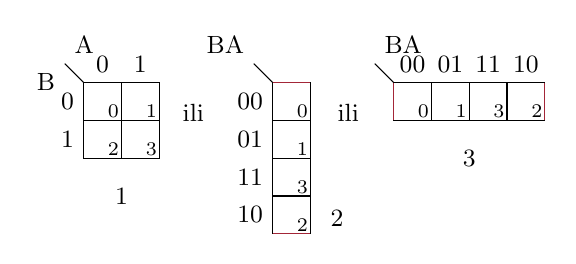
\begin{tikzpicture}[font=\fontsize{9}{10.5}\selectfont,x=4.8mm,y=4.8mm,
 DEindeks/.style={font=\fontsize{7}{8}\selectfont,anchor=south east,inner sep=.7pt}]
\draw (0,2) rectangle (2,4) (1,2)--(1,4) (0,3)--(2,3);
\draw (0,4)--(-.5,4.5) node[above right] {A} node[below left] {B};
\foreach \x/\lab in {.5/0,1.5/1}{\node[above] at (\x,4) {\lab};}
\foreach \y/\lab in {3.5/0,2.5/1}{\node[left] at (0,\y) {\lab};}
\foreach \x/\y/\lab in {1/3/0,2/3/1,1/2/2,2/2/3}{\node[DEindeks] at (\x,\y) {\lab};}
\node at (1,1) {1};
\node at (2.9,3.2) {ili};
\draw (5,0) rectangle (6,4);
\foreach \y in {1,2,3}{\draw (5,\y)--(6,\y);}
\draw (5,4)--(4.5,4.5) node[above left] {BA};
\foreach \y/\lab in {3.5/00,2.5/01,1.5/11,.5/10}{\node[left] at (5,\y) {\lab};}
\foreach \y/\lab in {3/0,2/1,1/3,0/2}{\node[DEindeks] at (6,\y) {\lab};}
\draw[DEcrvena] (5,0)--(6,0) (5,4)--(6,4);
\node at (6.7,.4) {2};
\node at (7,3.2) {ili};
\draw (8.2,3) rectangle (12.2,4);
\foreach \x in {9.2,10.2,11.2}{\draw (\x,3)--(\x,4);}
\draw (8.2,4)--(7.7,4.5) node[above right] {BA};
\foreach \x/\lab in {8.7/00,9.7/01,10.7/11,11.7/10}{\node[above] at (\x,4) {\lab};}
\foreach \x/\lab in {9.2/0,10.2/1,11.2/3,12.2/2}{\node[DEindeks] at (\x,3) {\lab};}
\draw[DEcrvena] (8.2,3)--(8.2,4) (12.2,3)--(12.2,4);
\node at (10.2,2) {3};
\end{tikzpicture}

\par\vspace{2mm}
\raggedright
\alert{Susedna polja imaju najmanje jednu zajedničku stranicu.}
\par\vspace{2mm}
Naspramne ivice karte se povezuju.
\end{column}
\end{columns}
\end{frame}

% Original: PDF strana 18, gornji slajd.
\slajdid{02-s035}
\begin{frame}[label=02-s035]{Karnoove karte za tri promenljive}
\setlength{\parskip}{0pt}
% element: 02-s035:e01
\begin{columns}[T,onlytextwidth]
\begin{column}{.47\textwidth}\centering
\Oznaka{Dve kolone i četiri reda}\vspace{1mm}
\begingroup
\fontsize{14.52}{16.13}\selectfont
\renewcommand{\small}{\fontsize{14.52}{16.13}\selectfont}
\scalebox{.62}{%
\begin{karnaugh-map}(label=middle)[2][4][1][$A$][$B$][$C$]
\foreach \x/\y/\lab in {1/3/0,2/3/1,1/2/2,2/2/3,1/1/6,2/1/7,1/0/4,2/0/5}{
 \node[anchor=south east,inner sep=1.1pt,font=\fontsize{11.29}{12.9}\selectfont] at (\x,\y) {\lab};
}
\end{karnaugh-map}}
\endgroup

\end{column}
\begin{column}{.47\textwidth}\centering
\Oznaka{Četiri kolone i dva reda}\vspace{1mm}
\begingroup
\fontsize{14.52}{16.13}\selectfont
\renewcommand{\small}{\fontsize{14.52}{16.13}\selectfont}
\scalebox{.62}{%
\begin{karnaugh-map}(label=middle)[4][2][1][$A$][$B$][$C$]
\foreach \x/\y/\lab in {1/1/0,2/1/1,3/1/3,4/1/2,1/0/4,2/0/5,3/0/7,4/0/6}{
 \node[anchor=south east,inner sep=1.1pt,font=\fontsize{11.29}{12.9}\selectfont] at (\x,\y) {\lab};
}
\end{karnaugh-map}}
\endgroup

\end{column}
\end{columns}
\par
% element: 02-s035:e02
U levoj karti susedna su i polja \(0\leftrightarrow4\) i \(1\leftrightarrow5\). To možemo zamisliti kao presavijanje tabele oko horizontalne ose po sredini i spajanje gornje i donje ivice u prsten.
\par\vspace{1mm}
U desnoj karti susedna su i polja \(0\leftrightarrow2\) i \(4\leftrightarrow6\). Ovde zamišljamo presavijanje oko vertikalne ose i spajanje leve i desne ivice u prsten.
\end{frame}

% Original: PDF strana 18, donji slajd.
\slajdid{02-s036}
\begin{frame}[label=02-s036]{Karnoova karta za četiri promenljive}
\setlength{\parskip}{0pt}
\begin{columns}[c,onlytextwidth]
\begin{column}{.48\textwidth}\centering
% element: 02-s036:e01
\begingroup
\def\DEskala{.74}\def\DEpomak{0}
% Zajednički raspored DC/BA. Parametri DEskala i DEpomak dolaze iz omotača.
% Nakon skaliranja oznake imaju 9 pt, indeksi 7 pt (odobren stil s034).
\pgfmathsetmacro{\DEfont}{9/\DEskala}
\pgfmathsetmacro{\DEindeksfont}{7/\DEskala}
\fontsize{\DEfont}{\DEfont}\selectfont
\renewcommand{\small}{\fontsize{\DEfont}{\DEfont}\selectfont}
\scalebox{\DEskala}{%
\begin{karnaugh-map}(label=middle)[4][4][1][$A$][$B$][$C$][$D$]
\foreach \x/\y/\base in {1/3/0,2/3/1,3/3/3,4/3/2,1/2/4,2/2/5,3/2/7,4/2/6,1/1/12,2/1/13,3/1/15,4/1/14,1/0/8,2/0/9,3/0/11,4/0/10}{
 \pgfmathtruncatemacro{\indeks}{\base+\DEpomak}
 \node[anchor=south east,inner sep=1pt,font=\fontsize{\DEindeksfont}{\DEindeksfont}\selectfont] at (\x,\y) {\indeks};
}
\end{karnaugh-map}}

\endgroup

\end{column}
\begin{column}{.48\textwidth}
% element: 02-s036:e02
Po definiciji jediničnog Hemingovog rastojanja, susedna polja razlikuju se u tačno jednom bitu. To važi i preko naspramnih ivica karte.
\par\vspace{3mm}
\Oznaka{Naspramne ivice su susedne}\par\vspace{1mm}
Vertikalno: \(0\leftrightarrow2\), \(4\leftrightarrow6\), \(12\leftrightarrow14\), \(8\leftrightarrow10\).
\par\vspace{2mm}
Horizontalno: \(0\leftrightarrow8\), \(1\leftrightarrow9\), \(3\leftrightarrow11\), \(2\leftrightarrow10\).
\end{column}
\end{columns}
\end{frame}

% Original: PDF strana 19, gornji slajd.
\slajdid{02-s037}
\begin{frame}[label=02-s037]{Karnoova karta za pet promenljivih}
\setlength{\parskip}{0pt}
% element: 02-s037:e01
\begin{columns}[T,onlytextwidth]
\begin{column}{.47\textwidth}\centering
\Oznaka{Sloj \(E=0\)}\par\vspace{1mm}
\begingroup
\def\DEskala{.68}\def\DEpomak{0}
% Zajednički raspored DC/BA. Parametri DEskala i DEpomak dolaze iz omotača.
% Nakon skaliranja oznake imaju 9 pt, indeksi 7 pt (odobren stil s034).
\pgfmathsetmacro{\DEfont}{9/\DEskala}
\pgfmathsetmacro{\DEindeksfont}{7/\DEskala}
\fontsize{\DEfont}{\DEfont}\selectfont
\renewcommand{\small}{\fontsize{\DEfont}{\DEfont}\selectfont}
\scalebox{\DEskala}{%
\begin{karnaugh-map}(label=middle)[4][4][1][$A$][$B$][$C$][$D$]
\foreach \x/\y/\base in {1/3/0,2/3/1,3/3/3,4/3/2,1/2/4,2/2/5,3/2/7,4/2/6,1/1/12,2/1/13,3/1/15,4/1/14,1/0/8,2/0/9,3/0/11,4/0/10}{
 \pgfmathtruncatemacro{\indeks}{\base+\DEpomak}
 \node[anchor=south east,inner sep=1pt,font=\fontsize{\DEindeksfont}{\DEindeksfont}\selectfont] at (\x,\y) {\indeks};
}
\end{karnaugh-map}}

\endgroup

\end{column}
\begin{column}{.47\textwidth}\centering
\Oznaka{Sloj \(E=1\)}\par\vspace{1mm}
\begingroup
\def\DEskala{.68}\def\DEpomak{16}
% Zajednički raspored DC/BA. Parametri DEskala i DEpomak dolaze iz omotača.
% Nakon skaliranja oznake imaju 9 pt, indeksi 7 pt (odobren stil s034).
\pgfmathsetmacro{\DEfont}{9/\DEskala}
\pgfmathsetmacro{\DEindeksfont}{7/\DEskala}
\fontsize{\DEfont}{\DEfont}\selectfont
\renewcommand{\small}{\fontsize{\DEfont}{\DEfont}\selectfont}
\scalebox{\DEskala}{%
\begin{karnaugh-map}(label=middle)[4][4][1][$A$][$B$][$C$][$D$]
\foreach \x/\y/\base in {1/3/0,2/3/1,3/3/3,4/3/2,1/2/4,2/2/5,3/2/7,4/2/6,1/1/12,2/1/13,3/1/15,4/1/14,1/0/8,2/0/9,3/0/11,4/0/10}{
 \pgfmathtruncatemacro{\indeks}{\base+\DEpomak}
 \node[anchor=south east,inner sep=1pt,font=\fontsize{\DEindeksfont}{\DEindeksfont}\selectfont] at (\x,\y) {\indeks};
}
\end{karnaugh-map}}

\endgroup

\end{column}
\end{columns}
\par\vspace{1mm}
% element: 02-s037:e02
\Oznaka{Susedstvo između slojeva}
Pored susedstva unutar svake karte, u 3D prostoru susedna su i polja koja se poklapaju pri preklapanju ove dve karte: \(0\leftrightarrow16\), \(1\leftrightarrow17\), itd.
\end{frame}

% Original: PDF strana 19, donji slajd.
\slajdid{02-s038}
\begin{frame}[label=02-s038]{Karnoova karta za šest promenljivih}
\setlength{\parskip}{0pt}
% element: 02-s038:e01
\begin{columns}[T,onlytextwidth]
\begin{column}{.24\textwidth}\centering
\Oznaka{\(FE=00\)}\par\vspace{1mm}
\begingroup
\def\DEpomak{0}
% DC/BA: isti indeksi kao u izvornim kartama; DEpomak bira sloj FE.
\begin{tikzpicture}[font=\fontsize{9}{10.5}\selectfont,x=5.6mm,y=5.6mm]
\draw[step=1,line width=.4pt] (0,0) grid (4,4);
\foreach \x/\lab in {.5/00,1.5/01,2.5/11,3.5/10}{\node[above,inner sep=1pt] at (\x,4) {\lab};}
\foreach \y/\lab in {3.5/00,2.5/01,1.5/11,.5/10}{\node[left,inner sep=1pt] at (0,\y) {\lab};}
\node[above] at (2,5) {\(BA\)};
\node[left] at (-.6,2) {\(DC\)};
\foreach \x/\y/\base in {.5/3.5/0,1.5/3.5/1,2.5/3.5/3,3.5/3.5/2,.5/2.5/4,1.5/2.5/5,2.5/2.5/7,3.5/2.5/6,.5/1.5/12,1.5/1.5/13,2.5/1.5/15,3.5/1.5/14,.5/.5/8,1.5/.5/9,2.5/.5/11,3.5/.5/10}{
 \pgfmathtruncatemacro{\indeks}{\base+\DEpomak}
 \node[anchor=south east,inner sep=.7pt,font=\fontsize{7}{8}\selectfont] at (\x+.5,\y-.5) {\indeks};
}
\end{tikzpicture}

\endgroup

\end{column}
\begin{column}{.24\textwidth}\centering
\Oznaka{\(FE=01\)}\par\vspace{1mm}
\begingroup
\def\DEpomak{16}
% DC/BA: isti indeksi kao u izvornim kartama; DEpomak bira sloj FE.
\begin{tikzpicture}[font=\fontsize{9}{10.5}\selectfont,x=5.6mm,y=5.6mm]
\draw[step=1,line width=.4pt] (0,0) grid (4,4);
\foreach \x/\lab in {.5/00,1.5/01,2.5/11,3.5/10}{\node[above,inner sep=1pt] at (\x,4) {\lab};}
\foreach \y/\lab in {3.5/00,2.5/01,1.5/11,.5/10}{\node[left,inner sep=1pt] at (0,\y) {\lab};}
\node[above] at (2,5) {\(BA\)};
\node[left] at (-.6,2) {\(DC\)};
\foreach \x/\y/\base in {.5/3.5/0,1.5/3.5/1,2.5/3.5/3,3.5/3.5/2,.5/2.5/4,1.5/2.5/5,2.5/2.5/7,3.5/2.5/6,.5/1.5/12,1.5/1.5/13,2.5/1.5/15,3.5/1.5/14,.5/.5/8,1.5/.5/9,2.5/.5/11,3.5/.5/10}{
 \pgfmathtruncatemacro{\indeks}{\base+\DEpomak}
 \node[anchor=south east,inner sep=.7pt,font=\fontsize{7}{8}\selectfont] at (\x+.5,\y-.5) {\indeks};
}
\end{tikzpicture}

\endgroup

\end{column}
\begin{column}{.24\textwidth}\centering
\Oznaka{\(FE=10\)}\par\vspace{1mm}
\begingroup
\def\DEpomak{32}
% DC/BA: isti indeksi kao u izvornim kartama; DEpomak bira sloj FE.
\begin{tikzpicture}[font=\fontsize{9}{10.5}\selectfont,x=5.6mm,y=5.6mm]
\draw[step=1,line width=.4pt] (0,0) grid (4,4);
\foreach \x/\lab in {.5/00,1.5/01,2.5/11,3.5/10}{\node[above,inner sep=1pt] at (\x,4) {\lab};}
\foreach \y/\lab in {3.5/00,2.5/01,1.5/11,.5/10}{\node[left,inner sep=1pt] at (0,\y) {\lab};}
\node[above] at (2,5) {\(BA\)};
\node[left] at (-.6,2) {\(DC\)};
\foreach \x/\y/\base in {.5/3.5/0,1.5/3.5/1,2.5/3.5/3,3.5/3.5/2,.5/2.5/4,1.5/2.5/5,2.5/2.5/7,3.5/2.5/6,.5/1.5/12,1.5/1.5/13,2.5/1.5/15,3.5/1.5/14,.5/.5/8,1.5/.5/9,2.5/.5/11,3.5/.5/10}{
 \pgfmathtruncatemacro{\indeks}{\base+\DEpomak}
 \node[anchor=south east,inner sep=.7pt,font=\fontsize{7}{8}\selectfont] at (\x+.5,\y-.5) {\indeks};
}
\end{tikzpicture}

\endgroup

\end{column}
\begin{column}{.24\textwidth}\centering
\Oznaka{\(FE=11\)}\par\vspace{1mm}
\begingroup
\def\DEpomak{48}
% DC/BA: isti indeksi kao u izvornim kartama; DEpomak bira sloj FE.
\begin{tikzpicture}[font=\fontsize{9}{10.5}\selectfont,x=5.6mm,y=5.6mm]
\draw[step=1,line width=.4pt] (0,0) grid (4,4);
\foreach \x/\lab in {.5/00,1.5/01,2.5/11,3.5/10}{\node[above,inner sep=1pt] at (\x,4) {\lab};}
\foreach \y/\lab in {3.5/00,2.5/01,1.5/11,.5/10}{\node[left,inner sep=1pt] at (0,\y) {\lab};}
\node[above] at (2,5) {\(BA\)};
\node[left] at (-.6,2) {\(DC\)};
\foreach \x/\y/\base in {.5/3.5/0,1.5/3.5/1,2.5/3.5/3,3.5/3.5/2,.5/2.5/4,1.5/2.5/5,2.5/2.5/7,3.5/2.5/6,.5/1.5/12,1.5/1.5/13,2.5/1.5/15,3.5/1.5/14,.5/.5/8,1.5/.5/9,2.5/.5/11,3.5/.5/10}{
 \pgfmathtruncatemacro{\indeks}{\base+\DEpomak}
 \node[anchor=south east,inner sep=.7pt,font=\fontsize{7}{8}\selectfont] at (\x+.5,\y-.5) {\indeks};
}
\end{tikzpicture}

\endgroup

\end{column}
\end{columns}
\par\vspace{3mm}
% element: 02-s038:e02
\Oznaka{Susedstvo između karata}
Pored susedstva unutar svake karte, u 4D prostoru susedna polja dobijamo i preklapanjem odgovarajućih karata: \(0\leftrightarrow32\), \(1\leftrightarrow33\), \(16\leftrightarrow48\), \(17\leftrightarrow49\), itd.
\end{frame}

% Original: PDF strana 20, gornji slajd.
\slajdid{02-s039}
\begin{frame}[label=02-s039]{Površine reda \(k\) u Karnoovoj karti}
% element: 02-s039:e01
\begin{center}
\begingroup\setlength{\tabcolsep}{10pt}
\begin{tabular}{c|rrrrrrr}
\toprule
Red \(k\) & 0 & 1 & 2 & 3 & 4 & 5 & 6 \\
\midrule
Broj susednih polja \(2^k\) & 1 & 2 & 4 & 8 & 16 & 32 & 64 \\
\bottomrule
\end{tabular}
\endgroup
\end{center}
\par\vspace{6mm}
% element: 02-s039:e02
\par\Rezultat{Površina mora biti pravilna: pravougaonik ili kvadrat u ravni, kvadar ili kocka u 3D, odgovarajući hiperkvadar u višoj dimenziji.}
\end{frame}

% Original: PDF strana 20, donji slajd.
\slajdid{02-s040}
\begin{frame}[label=02-s040]{Susedstvo preko ivica i između slojeva}
\setlength{\parskip}{0pt}
% element: 02-s040:e01
Kartu sa tri promenljive možemo zamisliti u 3D prostoru kao dve preklopljene karte: jednu za \(C=0\), a drugu za \(C=1\).
\par\vspace{1mm}
\begin{columns}[T,onlytextwidth]
\begin{column}{.30\textwidth}\centering
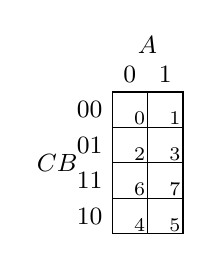
\begin{tikzpicture}[font=\fontsize{9}{10}\selectfont,x=4.5mm,y=4.5mm,baseline=(current bounding box.center)]
\draw (0,0) rectangle (2,4) (1,0)--(1,4);
\foreach \y in {1,2,3}{\draw (0,\y)--(2,\y);}
\node[above] at (1,4.8) {\(A\)};
\node[above] at (.5,4) {0};\node[above] at (1.5,4) {1};
\node[left] at (-.7,2) {\(CB\)};
\foreach \y/\lab in {3.5/00,2.5/01,1.5/11,.5/10}{\node[left] at (0,\y) {\lab};}
\foreach \x/\y/\lab in {1/3/0,2/3/1,1/2/2,2/2/3,1/1/6,2/1/7,1/0/4,2/0/5}{
 \node[anchor=south east,inner sep=.7pt,font=\fontsize{7}{8}\selectfont] at (\x,\y) {\lab};
}
\end{tikzpicture}

\end{column}
\begin{column}{.08\textwidth}\centering\vspace{15mm}\par \(=\)\end{column}
\begin{column}{.58\textwidth}\raggedright
% element: 02-s040:e03
% Zaglavlje C=1 usklađeno je s indeksima 4,5/6,7.
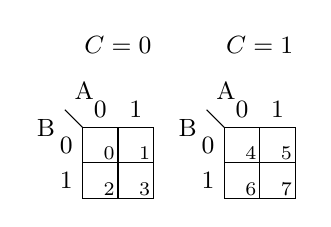
\begin{tikzpicture}[font=\fontsize{9}{10}\selectfont,x=4.5mm,y=4.5mm,baseline=(current bounding box.center)]
\draw (0,0) rectangle (2,2) (1,0)--(1,2) (0,1)--(2,1);
\draw (0,2)--(-.5,2.5) node[above right] {A} node[below left] {B};
\node[above] at (.5,2) {0};\node[above] at (1.5,2) {1};
\node[left] at (0,1.5) {0};\node[left] at (0,.5) {1};
\node[above] at (1,3.8) {\(C=0\)};
\foreach \x/\y/\lab in {1/1/0,2/1/1,1/0/2,2/0/3}{
 \node[anchor=south east,inner sep=1pt,font=\fontsize{7}{8}\selectfont] at (\x,\y) {\lab};
}
\draw (4,0) rectangle (6,2) (5,0)--(5,2) (4,1)--(6,1);
\draw (4,2)--(3.5,2.5) node[above right] {A} node[below left] {B};
\node[above] at (4.5,2) {0};\node[above] at (5.5,2) {1};
\node[left] at (4,1.5) {0};\node[left] at (4,.5) {1};
\node[above] at (5,3.8) {\(C=1\)};
\foreach \x/\y/\lab in {5/1/4,6/1/5,5/0/6,6/0/7}{
 \node[anchor=south east,inner sep=1pt,font=\fontsize{7}{8}\selectfont] at (\x,\y) {\lab};
}
\end{tikzpicture}

\end{column}
\end{columns}
\par\vspace{3mm}
% element: 02-s040:e02
\begin{columns}[T,onlytextwidth]
\begin{column}{.48\textwidth}
\begin{minipage}[c]{.61\linewidth}\raggedright
\Oznaka{Površina 1. reda}\par\vspace{1mm}
U 3D preklapanju susedna su polja \(0\) i \(4\), \(1\) i \(5\), itd. Zato je i grupa \(0,4\) pravilna površina 1. reda.
\end{minipage}\hfill
\begin{minipage}[c]{.36\linewidth}\centering
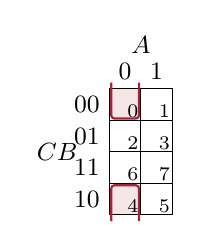
\begin{tikzpicture}[font=\fontsize{9}{10}\selectfont,x=4mm,y=4mm,baseline=(current bounding box.center)]
\fill[DEcrvena!12] (.06,3.06) rectangle (0.94,4);
\fill[DEcrvena!12] (.06,0) rectangle (0.94,.94);
\draw (0,0) rectangle (2,4) (1,0)--(1,4);
\foreach \y in {1,2,3}{\draw (0,\y)--(2,\y);}
\node[above] at (1,4.8) {\(A\)};
\node[above] at (.5,4) {0};\node[above] at (1.5,4) {1};
\node[left] at (-.7,2) {\(CB\)};
\foreach \y/\lab in {3.5/00,2.5/01,1.5/11,.5/10}{\node[left] at (0,\y) {\lab};}
\foreach \x/\y/\lab in {1/3/0,2/3/1,1/2/2,2/2/3,1/1/6,2/1/7,1/0/4,2/0/5}{
 \node[anchor=south east,inner sep=.7pt,font=\fontsize{7}{8}\selectfont] at (\x,\y) {\lab};
}
\draw[DEcrvena,line width=.8pt,rounded corners=.4mm] (.06,4.2)--(.06,3.06)--(0.94,3.06)--(0.94,4.2);
\draw[DEcrvena,line width=.8pt,rounded corners=.4mm] (.06,-.2)--(.06,.94)--(0.94,.94)--(0.94,-.2);
\end{tikzpicture}

\end{minipage}
\end{column}
\begin{column}{.48\textwidth}
\begin{minipage}[c]{.61\linewidth}\raggedright
\Oznaka{Površina 2. reda}\par\vspace{1mm}
Pravilna površina 2. reda može prekrivati i polja \(0,1,4,5\), preko gornje i donje ivice karte.
\end{minipage}\hfill
\begin{minipage}[c]{.36\linewidth}\centering
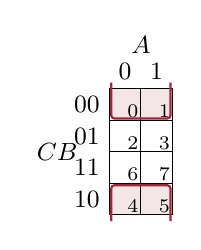
\begin{tikzpicture}[font=\fontsize{9}{10}\selectfont,x=4mm,y=4mm,baseline=(current bounding box.center)]
\fill[DEcrvena!12] (.06,3.06) rectangle (1.94,4);
\fill[DEcrvena!12] (.06,0) rectangle (1.94,.94);
\draw (0,0) rectangle (2,4) (1,0)--(1,4);
\foreach \y in {1,2,3}{\draw (0,\y)--(2,\y);}
\node[above] at (1,4.8) {\(A\)};
\node[above] at (.5,4) {0};\node[above] at (1.5,4) {1};
\node[left] at (-.7,2) {\(CB\)};
\foreach \y/\lab in {3.5/00,2.5/01,1.5/11,.5/10}{\node[left] at (0,\y) {\lab};}
\foreach \x/\y/\lab in {1/3/0,2/3/1,1/2/2,2/2/3,1/1/6,2/1/7,1/0/4,2/0/5}{
 \node[anchor=south east,inner sep=.7pt,font=\fontsize{7}{8}\selectfont] at (\x,\y) {\lab};
}
\draw[DEcrvena,line width=.8pt,rounded corners=.4mm] (.06,4.2)--(.06,3.06)--(1.94,3.06)--(1.94,4.2);
\draw[DEcrvena,line width=.8pt,rounded corners=.4mm] (.06,-.2)--(.06,.94)--(1.94,.94)--(1.94,-.2);
\end{tikzpicture}

\end{minipage}
\end{column}
\end{columns}
\end{frame}

% Original: PDF strana 21, gornji slajd.
\slajdid{02-s041}
\begin{frame}[label=02-s041]{Algoritam minimizacije}
\setlength{\parskip}{0pt}
% element: 02-s041:e01
Iz funkcionalne tabele ili specifikacije kombinacione mreže unosimo vrednosti funkcije u odgovarajuća polja Karnoove karte, prema stanjima ulaznih promenljivih.
\par\vspace{1.5mm}
% element: 02-s041:e02
\begin{enumerate}
\item Za funkciju u obliku \textbf{zbira proizvoda}, sve logičke jedinice u karti treba prekriti \alert{što manjim brojem površina što višeg reda}.
\item Za funkciju u obliku \textbf{proizvoda zbirova}, sve logičke nule u karti treba prekriti \alert{što manjim brojem površina što višeg reda}.
\end{enumerate}
\par\vspace{2mm}
% element: 02-s041:e03
\Oznaka{Uslov minimalnosti}\par\vspace{1mm}
Ako je broj površina minimalan, a površine najveće moguće, algoritam garantuje minimalnu funkciju. Pod tim uslovom nije moguća jednostavnija realizacija pomoću I i ILI logičkih kola.
\par\vspace{1.5mm}
\Rezultat{Podrazumevamo da su na ulazu kombinacione mreže dostupne i prave i komplementne vrednosti signala.}
\end{frame}

% Original: PDF strana 21, donji slajd.
\slajdid{02-s042}
\begin{frame}[label=02-s042]{Neodređena stanja i stalni literali}
\setlength{\parskip}{0pt}
% element: 02-s042:e01
\Oznaka{Proizvoljna vrednost: \(b\) ili \(X\)}\par\vspace{1mm}
Ako funkcija u nekom polju može imati bilo koju vrednost, to polje u minimizaciji koristimo kao \textbf{logičku jedinicu ili logičku nulu}, da dobijemo što jednostavniju formu.
\par\vspace{1mm}
Na primer, za zbir proizvoda možemo ga koristiti kao jedinicu, a za proizvod zbirova kao nulu, ili obrnuto --- prema tome šta omogućava povoljnije sažimanje.
\par\vspace{3mm}
% element: 02-s042:e02
Površine objedinjuju proizvode koje je moguće sažeti na prethodno opisani način.
\par\vspace{2mm}
\begin{columns}[T,onlytextwidth]
\begin{column}{.48\textwidth}
\Oznaka{Zbir proizvoda}\par\vspace{1mm}
Ostaju literali koji se \alert{\textbf{ne menjaju}} na površini.
\end{column}
\begin{column}{.48\textwidth}
\Oznaka{Proizvod zbirova}\par\vspace{1mm}
Ostaju \alert{\textbf{komplementi literala}} koji se \alert{\textbf{ne menjaju}} na površini.
\end{column}
\end{columns}
\par\vspace{3mm}
% element: 02-s042:e03
\Rezultat{Promenljive koje se menjaju na površini ne pojavljuju se u odgovarajućem proizvodu ili zbiru.}
\end{frame}

% Original: PDF strana 22, gornji slajd.
\slajdid{02-s043}
\begin{frame}[label=02-s043]{Primer: minimalni zbir proizvoda}
\setlength{\parskip}{0pt}
Na osnovu zahteva za kombinacionom mrežom formirana je polazna Karnoova tabela.
\par\vspace{1.5mm}
\begin{columns}[T,onlytextwidth]
\begin{column}{.29\textwidth}\centering
% element: 02-s043:e01
\Oznaka{Polazna karta}\par\vspace{2mm}
% Bitovi indeksa su DCBA; kolone BA=00,01,11,10, redovi DC=00,01,11,10.
\begingroup
\fontsize{16.67}{18.5}\selectfont
\renewcommand{\small}{\fontsize{16.67}{18.5}\selectfont}
\scalebox{.54}{%
\begin{karnaugh-map}(label=middle)[4][4][1][$A$][$B$][$C$][$D$]
\minterms{0,4,5,8,10}
\terms{1}{b}
\maxterms{2,3,6,7,9,11,12,13,14,15}
\end{karnaugh-map}
}
\endgroup

\end{column}
\begin{column}{.29\textwidth}\centering
% element: 02-s043:e03
\Oznaka{Pokrivanje jedinica}\par\vspace{2mm}
\begingroup
\fontsize{16.67}{18.5}\selectfont
\renewcommand{\small}{\fontsize{16.67}{18.5}\selectfont}
\scalebox{.54}{%
\begin{karnaugh-map}(label=middle,implicantcolors={DEcrvena,DEcrvena,DEcrvena})[4][4][1][$A$][$B$][$C$][$D$]
\minterms{0,4,5,8,10}
\terms{1}{b}
\maxterms{2,3,6,7,9,11,12,13,14,15}
\implicant{0}{5}
{\tikzset{every path/.append style={dashed}}\implicantedge{8}{8}{10}{10}}
\end{karnaugh-map}
}
\endgroup

\end{column}
\begin{column}{.38\textwidth}
% element: 02-s043:e02
Za minimalnu funkciju u obliku zbira proizvoda prekrivamo sve logičke jedinice površinama najvišeg reda, koristeći po potrebi i neodređeno stanje \(b\).
\par\vspace{1.5mm}
Površine objedinjuju proizvode koji se mogu sažeti. U proizvodima ostaju samo literali koji se \alert{\textbf{ne menjaju}} na površini.
\end{column}
\end{columns}
\par\vspace{2mm}
% element: 02-s043:e04
\par\Rezultat{\(F=\bar D\bar B+D\bar C\bar A\)}
\end{frame}

% Original: PDF strana 22, donji slajd.
\slajdid{02-s044}
\begin{frame}[label=02-s044]{Primer: minimalni proizvod zbirova}
\setlength{\parskip}{0pt}
% element: 02-s044:e01
Za minimalnu funkciju u obliku proizvoda zbirova prekrivamo sve logičke nule površinama najvišeg reda, koristeći po potrebi i neodređeno stanje \(b\).
\par\vspace{2mm}
\begin{columns}[T,onlytextwidth]
\begin{column}{.39\textwidth}\centering
% element: 02-s044:e02
% Original prikazuje samo grupu celog reda DC=11; ostale grupe se ne dopisuju.
\begingroup
\fontsize{12}{13.3}\selectfont
\renewcommand{\small}{\fontsize{12}{13.3}\selectfont}
\scalebox{.75}{%
\begin{karnaugh-map}(label=middle,implicantcolors={DEcrvena,DEcrvena,DEcrvena})[4][4][1][$A$][$B$][$C$][$D$]
\minterms{0,4,5,8,10}
\terms{1}{b}
\maxterms{2,3,6,7,9,11,12,13,14,15}
\implicant{12}{14}
\end{karnaugh-map}}
\endgroup

\end{column}
\begin{column}{.57\textwidth}
% element: 02-s044:e03
Površine objedinjuju kombinacije za koje je moguće sažimanje izraza.
\par\vspace{2mm}
U zbirovima ostaju \alert{\textbf{komplementi literala}} koji se \alert{\textbf{ne menjaju}} na površini.
\par\vspace{5mm}
% element: 02-s044:e04
\par\Rezultat{\(F=(D+\bar B)(\bar D+\bar C)(\bar D+\bar A)\)}
\end{column}
\end{columns}
\end{frame}

% Original: PDF strana 23, gornji slajd.
\slajdid{02-s045}
\begin{frame}[label=02-s045]{Poređenje po broju ulaza kola}
\setlength{\parskip}{0pt}
% element: 02-s045:e01
\begin{columns}[T,onlytextwidth]
\begin{column}{.48\textwidth}
\Oznaka{Zbir proizvoda}
\[F=\bar D\bar B+D\bar C\bar A\]
Jedno dvoulazno I, jedno troulazno I i jedno dvoulazno ILI kolo.
\[2+3+2=\mathbf{7}\text{ ulaza}\]
\end{column}
\begin{column}{.48\textwidth}
\Oznaka{Proizvod zbirova}
\[F=(D+\bar B)(\bar D+\bar C)(\bar D+\bar A)\]
Tri dvoulazna ILI i jedno troulazno I kolo.
\[3\cdot2+3=\mathbf{9}\text{ ulaza}\]
\end{column}
\end{columns}
\par\vspace{3mm}
% element: 02-s045:e02
Za ovaj primer zbir proizvoda je povoljniji prema ukupnom broju ulaza I i ILI kola.
\par\vspace{2mm}
\Rezultat{\alert{\textbf{Unapred se ne zna koja je realizacija povoljnija.}} Treba izvesti \alert{\textbf{oba minimalna izraza}} — zbir proizvoda i proizvod zbirova — pa njihovim poređenjem zaključiti koja je realizacija minimalna prema izabranom kriterijumu.}
\end{frame}

% Original: PDF strana 23, donji slajd.
\slajdid{02-s046}
\begin{frame}[label=02-s046]{Ista funkcija: drugačiji broj čipova}
\setlength{\parskip}{0pt}
\renewcommand{\arraystretch}{1.0}
Međutim, pri poređenju po broju čipova rezultat može biti drugačiji ili isti.
\par\vspace{1.5mm}
U oba oblika potrebna su četiri invertora za \(\bar D,\bar C,\bar B,\bar A\).
\par\vspace{1.5mm}
% element: 02-s046:e01
\begin{columns}[T,onlytextwidth]
\begin{column}{.48\textwidth}
\Oznaka{Zbir proizvoda — ukupno \textbf{4 čipa}}\Oznaka{\(F=\bar D\bar B+D\bar C\bar A\)}
\par\vspace{1.5mm}
\begin{tabular}{@{}ll@{}}
4 invertora & 1 čip \\
1 dvoulazno I & 1 čip \\
1 troulazno I & 1 čip \\
1 dvoulazno ILI & 1 čip \\
\end{tabular}

\end{column}
\begin{column}{.48\textwidth}
% element: 02-s046:e02
\Oznaka{Proizvod zbirova — ukupno \textbf{3 čipa}}\Oznaka{\(F=(D+\bar B)(\bar D+\bar C)(\bar D+\bar A)\)}
\par\vspace{1.5mm}
\begin{tabular}{@{}ll@{}}
4 invertora & 1 čip \\
3 dvoulazna ILI & 1 čip \\
1 troulazno I & 1 čip \\
\end{tabular}

\end{column}
\end{columns}
\par\vspace{1.5mm}
U 14-pinskom kućištu dva pina služe za masu i napajanje, pa ostaje 12 signalnih pinova:
\par
Invertor: 1 ulaz + 1 izlaz \(\Rightarrow (14-2)/2=6\) invertora u jednom čipu.
\par
Dvoulazno ILI: 2 ulaza + 1 izlaz \(\Rightarrow (14-2)/3=4\) kola u jednom čipu.
\par\vspace{1.5mm}
% element: 02-s046:e03
\alert{\textbf{Prema broju čipova povoljniji je proizvod zbirova}}, iako ima više ulaza kola.
\end{frame}

% Original: PDF strana 24, gornji slajd.
\slajdid{02-s047}
\begin{frame}[label=02-s047]{Grupisanje proizvoda i broj čipova}
\setlength{\parskip}{0pt}
Algebarskom preraspodelom proizvoda možemo realizovati istu funkciju pomoću dvoulaznih I kola, uz povećano kašnjenje:
% element: 02-s047:e01
\[F=\bar D\bar B+D\bar C\bar A=\bar D\bar B+(D\bar C)\bar A\]
\par\vspace{3mm}
% element: 02-s047:e02
Za ovu realizaciju potrebni su:
\begin{itemize}
\item jedan čip sa invertorima;
\item jedan čip sa dvoulaznim I kolima — koristimo \textbf{tri I kola}, koja se nalaze u jednom čipu;
\item jedan čip sa dvoulaznim ILI kolima.
\end{itemize}
\par\vspace{2mm}
% element: 02-s047:e03
\Rezultat{Ukupno \textbf{3 čipa}. Troulazni proizvod realizujemo kaskadom dva dvoulazna I kola: smanjujemo broj potrebnih kućišta, \alert{\textbf{na račun povećanog kašnjenja}}.}
\end{frame}

% Original: PDF strana 24, donji slajd.
\slajdid{02-s048}
\begin{frame}[label=02-s048]{NI realizacija: tri različite vrste čipova}
\setlength{\parskip}{0pt}
Da bismo koristili kola iste vrste, funkciju najčešće algebarski preoblikujemo za realizaciju NI ili NILI kolima. Za NI realizaciju po pravilu je najlakše poći od zbira proizvoda:
% element: 02-s048:e01
\[F=\bar D\bar B+D\bar C\bar A
=\overline{\overline{\bar D\bar B+D\bar C\bar A}}
=\overline{\overline{\bar D\bar B}\cdot\overline{D\bar C\bar A}}\]
\par\vspace{2mm}
% element: 02-s048:e02
Potrebni su:
\begin{itemize}
\item jedan čip sa najmanje \textbf{četiri invertora};
\item jedan čip sa najmanje \textbf{dva dvoulazna NI kola};
\item jedan čip sa najmanje \textbf{jednim troulaznim NI kolom}.
\end{itemize}
Ukupno su to \textbf{tri čipa različitih vrsta}.
\par\vspace{3mm}
% element: 02-s048:e04
\Rezultat{NI transformacija \alert{\textbf{ne dokazuje minimalnost}} prema klasičnoj minimizaciji.}
\end{frame}

% Original: PDF strana 24, donji slajd; odobren drugi deo s048.
\slajdid{02-s048b}
\begin{frame}[label=02-s048b]{Dvoulazna NI kola: tri ili dva čipa?}
\setlength{\parskip}{0pt}
% element: 02-s048b:e01
Zamena troulaznog NI kola: dva dvoulazna NI i invertor, \alert{\textbf{uz povećano kašnjenje}}:
\par\vspace{2mm}
{\centering\(\displaystyle\overline{XYZ}=\overline{(XY)Z}
=\overline{\overline{\overline{XY}}\,Z}.\)\par}
\vspace{2mm}
\begin{columns}[T,onlytextwidth]
\begin{column}{.48\textwidth}
% element: 02-s048b:e02
\Oznaka{Samo dvoulazna NI kola}
\begin{itemize}
\setlength{\itemsep}{1pt}\setlength{\parsep}{0pt}
\item 4 NI kola za četiri ulazne inverzije;
\item 3 NI kola za zamenu troulaznog NI;
\item još 2 NI kola za ostatak funkcije.
\end{itemize}
\(4+3+2=9\) dvoulaznih NI kola.\par
Četiri kola po čipu: \textbf{3 ista čipa}.
\end{column}
\begin{column}{.48\textwidth}
% element: 02-s048b:e03
\Oznaka{Čip sa invertorima + čip sa NI kolima}
Čip sa šest invertora:\par
4 za ulazne komplemente;\par
1 od dva preostala za međuinverziju.
\par\vspace{1.5mm}
Čip sa četiri dvoulazna NI kola:\par
\textbf{sva četiri kola za funkciju}.
\par\vspace{1.5mm}
Ukupno: \textbf{2 čipa različitih vrsta}.
\end{column}
\end{columns}
\par\vspace{2mm}
% element: 02-s048b:e04
\Rezultat{Tri ista čipa mogu doneti popust na količinu. Da li je jeftinije \textbf{1 + 1 različitih čipova ili 3 ista}? \alert{\textbf{Nema opšteg odgovora}} — zavisi od cena i uslova nabavke.}
\end{frame}

% Original: PDF strana 25, gornji slajd; odobren prvi deo s049.
\slajdid{02-s049}
\begin{frame}[label=02-s049]{NILI realizacija: tri različite vrste čipova}
\setlength{\parskip}{0pt}
% element: 02-s049:e01
Za realizaciju NILI kolima po pravilu je najlakše poći od proizvoda zbirova:
\[\begin{aligned}
F&=\textcolor{DEcrvena}{(D+\bar B)(\bar D+\bar C)(\bar D+\bar A)}\\[1.5mm]
 &=\overline{\overline{(D+\bar B)(\bar D+\bar C)(\bar D+\bar A)}}
 =\overline{\overline{(D+\bar B)}+\overline{(\bar D+\bar C)}+\overline{(\bar D+\bar A)}}.
\end{aligned}\]
% element: 02-s049:e02
Potrebni su:
\begin{itemize}
\item jedan čip sa najmanje \textbf{četiri invertora};
\item jedan čip sa najmanje \textbf{tri dvoulazna NILI kola};
\item jedan čip sa najmanje \textbf{jednim troulaznim NILI kolom}.
\end{itemize}
Ukupno su to \textbf{tri čipa različitih vrsta}.
\par\vspace{2mm}
% element: 02-s049:e04
\Rezultat{Ni ova NILI transformacija \alert{\textbf{ne dokazuje minimalnost}} prema klasičnoj minimizaciji.}
\end{frame}

% Original: PDF strana 25, gornji slajd; odobren drugi deo s049.
\slajdid{02-s049b}
\begin{frame}[label=02-s049b]{Dvoulazna NILI kola i složena CMOS realizacija}
\setlength{\parskip}{0pt}
% element: 02-s049b:e01
Troulazno NILI kolo zamenjujemo sa dva dvoulazna NILI kola i invertorom:
\par\vspace{2mm}
{\centering\(\displaystyle\overline{X+Y+Z}=\overline{(X+Y)+Z}
=\overline{\overline{\overline{X+Y}}+Z}.\)\par}
\par\vspace{3mm}
% element: 02-s049b:e02
Za realizaciju samo dvoulaznim NILI kolima potrebni su:
\begin{itemize}
\item 4 kola za ulazne inverzije — NILI sa spojenim ulazima;
\item 3 kola za zamenu troulaznog NILI, uključujući međuinverziju;
\item 3 kola za preostali deo funkcije.
\end{itemize}
Ukupno: \(4+3+3=10\) dvoulaznih NILI kola. Četiri kola po čipu: \textbf{3 ista čipa}.
\par\vspace{3mm}
% element: 02-s049b:e03
\Rezultat{\textbf{Probajte:} uz raspoložive \alert{\textbf{komplementne vrednosti ulaza}}, uporedite oba oblika funkcije kao \alert{\textbf{jednostepena složena CMOS kola}}. Koja realizacija zauzima \alert{\textbf{manju površinu}}?}
\end{frame}

% Original: PDF strana 25, donji slajd.
\slajdid{02-s050}
\begin{frame}[label=02-s050]{Lažne nule i jedinice — glič}
\setlength{\parskip}{0pt}
% element: 02-s050:e01
Kašnjenja logičkih kola razlikuju se i zavise od fabrikacije, temperature, starosti komponenti i drugih uslova. Zato se pri promeni ulaznih signala mogu pojaviti neželjeni efekti na izlazu.
\par\vspace{2mm}
\begin{columns}[T,onlytextwidth]
\begin{column}{.48\textwidth}
\Oznaka{Lažna nula}
Izlaz je 1 i posle promene ulaza treba da ostane 1. Zbog prostiranja signala ipak se pojavi \alert{\textbf{kratkotrajna nula}}.
\end{column}
\begin{column}{.48\textwidth}
\Oznaka{Lažna jedinica}
Izlaz je 0 i posle promene ulaza treba da ostane 0. Zbog prostiranja signala ipak se pojavi \alert{\textbf{kratkotrajna jedinica}}.
\end{column}
\end{columns}
\par\vspace{2mm}
Ovi kratkotrajni neželjeni impulsi nazivaju se \alert{\textbf{glič}} (engl. \emph{glitch}).
\par\vspace{1mm}
% element: 02-s050:e02
\Oznaka{Posmatrajmo primer kombinacione mreže: \(F=C\bar B+BA\).}
{\centering\begin{tikzpicture}[circuit logic US,DEoznaka,x=1cm,y=1cm,
 gate/.style={draw,logic gate inputs=nn,minimum width=12mm,minimum height=9mm,scale=.6}]
\node[and gate US,gate] (u) at (2,1.1) {};
\node[and gate US,gate] (d) at (2,-.1) {};
\node[or gate US,gate] (f) at (3.8,.5) {};
\node[not gate US,draw,minimum width=8mm,minimum height=8mm,scale=.6] (i) at (.6,.55) {};
\draw[DEvod] (u.input 1)--(-.5,0 |- u.input 1) node[left] {$C$};
\draw[DEvod] (i.input)--(-.5,.55) node[left] {$B$};
\draw[DEvod] (i.output)--(1.25,.55)|-(u.input 2);
\draw[DEvod] (-.2,.55)|-(d.input 1);
\node[junction] at (-.2,.55) {};
\draw[DEvod] (d.input 2)--(-.5,0 |- d.input 2) node[left] {$A$};
\draw[DEvod] (u.output)--(2.8,1.1)|-(f.input 1);
\draw[DEvod] (d.output)--(2.8,-.1)|-(f.input 2);
\draw[DEvod] (f.output)--++(.4,0) node[right] {$F$};
\end{tikzpicture}
\par}
\end{frame}

% Original: PDF strana 26, gornji slajd.
\slajdid{02-s051}
\begin{frame}[label=02-s051]{Statički hazard: izlaz treba da ostane 1}
\setlength{\parskip}{0pt}
% element: 02-s051:e01
Radi uočavanja pojave pretpostavljamo da su sva kola idealno brza, osim invertora, čije je kašnjenje \(t_p\).
\par\vspace{2mm}
\begin{columns}[T,onlytextwidth]
\begin{column}{.52\textwidth}
% element: 02-s051:e02
{\centering\begin{tikzpicture}[circuit logic US,DEoznaka,x=1cm,y=1cm,
 gate/.style={draw,logic gate inputs=nn,minimum width=12mm,minimum height=9mm,scale=.6}]
\node[and gate US,gate] (u) at (2,1.1) {};
\node[and gate US,gate] (d) at (2,-.1) {};
\node[or gate US,gate] (f) at (3.8,.5) {};
\node[not gate US,draw,minimum width=8mm,minimum height=8mm,scale=.6] (i) at (.6,.55) {};
\draw[DEvod] (u.input 1)--(-.5,0 |- u.input 1) node[left] {$C$};
\draw[DEvod] (i.input)--(-.5,.55) node[left] {$B$};
\draw[DEvod] (i.output)--(1.25,.55)|-(u.input 2);
\draw[DEvod] (-.2,.55)|-(d.input 1);
\node[junction] at (-.2,.55) {};
\draw[DEvod] (d.input 2)--(-.5,0 |- d.input 2) node[left] {$A$};
\draw[DEvod] (u.output)--(2.8,1.1)|-(f.input 1);
\draw[DEvod] (d.output)--(2.8,-.1)|-(f.input 2);
\draw[DEvod] (f.output)--++(.4,0) node[right] {$F$};
\end{tikzpicture}
\par}
\par\vspace{2mm}
Početno stanje: \(C=B=A=1\), pa je \(F=C\bar B+BA=1\).
\par\vspace{1mm}
Menja se samo \(B:1\to0\). Konačno stanje: \(C=A=1\), \(B=0\), pa je opet \(F=1\).
\par\vspace{1mm}
Izlaz \textbf{treba da ostane 1}, \alert{\textbf{ali}} tokom prelaza javlja se \alert{\textbf{lažna nula}}.
\end{column}
\begin{column}{.43\textwidth}\centering
% element: 02-s051:e03
% Kompaktan vektorski dijagram; logičke vrednosti i redosled događaja su iz originala.
\begin{tikzpicture}[x=1cm,y=1cm,font=\fontsize{9}{10.5}\selectfont]
\foreach \r/\lab in {0/A,1/B,2/{\bar B},3/C,4/A,5/{BA},6/{C\bar B},7/F}{
 \pgfmathsetmacro{\yy}{-.50*\r}
 \draw[black!55,thin,-{Latex[length=.9mm]}] (0,\yy-.03)--(0,\yy+.39) node[left] {$\lab$};
 \draw[black!55,thin,-{Latex[length=.9mm]}] (-.08,\yy)--(3.72,\yy) node[below] {$t$};
}
\foreach \r in {0,3,4}{
 \pgfmathsetmacro{\yy}{-.50*\r}
 \draw[DEvod] (0,\yy+.32)--(3.35,\yy+.32);
}
\foreach \r in {1,5}{
 \pgfmathsetmacro{\yy}{-.50*\r}
 \draw[DEvod] (0,\yy+.32)--(.95,\yy+.32)--(1.06,\yy+.10)--(3.35,\yy+.10);
}
\foreach \r in {2,6}{
 \pgfmathsetmacro{\yy}{-.50*\r}
 \draw[DEvod] (0,\yy+.10)--(1.76,\yy+.10)--(1.88,\yy+.32)--(3.35,\yy+.32);
}
\draw[DEvod] (0,-3.18)--(.95,-3.18)--(1.06,-3.40)--(1.76,-3.40)--(1.88,-3.18)--(3.35,-3.18);
% Trajanje je iznad svih signala, da strelica ne seče talasne oblike.
\draw[DEvod,dashed] (1,.63)--(1,-3.57);
\draw[DEvod,dashed] (1.82,.63)--(1.82,-3.57);
\draw[DEvod,{Latex[length=1.1mm]}-{Latex[length=1.1mm]}] (1,.72)--(1.82,.72)
 node[midway,above,inner sep=1pt] {$t_p$};
\node[inner sep=1pt] at (2.7,-3.83) {lažna nula};
\end{tikzpicture}

\end{column}
\end{columns}
\end{frame}

% Original: PDF strana 26, donji slajd.
\slajdid{02-s052}
\begin{frame}[label=02-s052]{Minimizacija i prelaz između površina}
% element: 02-s052:e01
\Rezultat{\(\textcolor{DEcrvena}{F=\bar C\bar B+BA}\)}
\par\vspace{4mm}
% element: 02-s052:e02
\begin{columns}[T,onlytextwidth]
\begin{column}{.30\textwidth}\centering
\Oznaka{Član \(\bar C\bar B\)}\vspace{4mm}
% Izvorne karte su očuvane; formula je usklađena po korisnikovoj odluci.
\begingroup
\fontsize{16.364}{18.2}\selectfont
\renewcommand{\small}{\fontsize{16.364}{18.2}\selectfont}
\scalebox{.55}{%
\begin{karnaugh-map}(label=middle,implicantcolors={DEcrvena,DEcrvena,DEcrvena})[4][2][1][$A$][$B$][$C$]
\terms{0,1,2,3,4,5,6,7}{\strut}
\implicant{0}{1}
\end{karnaugh-map}}
\endgroup

\end{column}
\begin{column}{.30\textwidth}\centering
\Oznaka{Član \(BA\)}\vspace{4mm}
% Izvorne karte su očuvane; formula je usklađena po korisnikovoj odluci.
\begingroup
\fontsize{16.364}{18.2}\selectfont
\renewcommand{\small}{\fontsize{16.364}{18.2}\selectfont}
\scalebox{.55}{%
\begin{karnaugh-map}(label=middle,implicantcolors={DEcrvena,DEcrvena,DEcrvena})[4][2][1][$A$][$B$][$C$]
\terms{0,1,2,3,4,5,6,7}{\strut}
\implicant{3}{7}
\end{karnaugh-map}}
\endgroup

\end{column}
\begin{column}{.34\textwidth}\centering
\Oznaka{Karta funkcije}\vspace{4mm}
% Izvorne karte su očuvane; formula je usklađena po korisnikovoj odluci.
\begingroup
\fontsize{16.364}{18.2}\selectfont
\renewcommand{\small}{\fontsize{16.364}{18.2}\selectfont}
\scalebox{.55}{%
\begin{karnaugh-map}(label=middle,implicantcolors={DEcrvena,DEcrvena,DEcrvena})[4][2][1][$A$][$B$][$C$]
\minterms{0,1,3,7}\maxterms{2,4,5,6}
\implicant{0}{1}
\end{karnaugh-map}}
\endgroup

\end{column}
\end{columns}
\par\vspace{5mm}
Za promenljive \(C,B,A\), funkcija nastaje minimizacijom potpunog oblika prikazanog u Karnoovoj karti.
\end{frame}

% Original: PDF strana 27, gornji slajd.
\slajdid{02-s053}
\begin{frame}[label=02-s053]{Povezivanje površina: uklanjanje lažne nule}
\setlength{\parskip}{0pt}
\begin{columns}[T,onlytextwidth]
\begin{column}{.31\textwidth}\centering
\Oznaka{Bez zajedničkog polja}\vspace{1mm}
% Izvorne karte su očuvane; formula je usklađena po korisnikovoj odluci.
\begingroup
\fontsize{16.364}{18.2}\selectfont
\renewcommand{\small}{\fontsize{16.364}{18.2}\selectfont}
\scalebox{.55}{%
\begin{karnaugh-map}(label=middle,implicantcolors={DEcrvena,DEcrvena,DEcrvena})[4][2][1][$A$][$B$][$C$]
\minterms{0,1,3,7}\maxterms{2,4,5,6}
{\tikzset{every path/.append style={dashed}}\implicant{0}{1}}
{\tikzset{every path/.append style={dashed}}\implicant{3}{7}}
\end{karnaugh-map}}
\endgroup

\end{column}
\begin{column}{.63\textwidth}
% element: 02-s053:e01
Dve minimizovane površine imaju zajedničku stranu, ali \alert{\textbf{nemaju zajednička polja}}: na prvoj je \(B=0\), na drugoj \(B=1\).\par\vspace{1mm}
Susedni prelaz \(B:1\to0\), pri \(C=0\), \(A=1\), menja samo jednu promenljivu. Različita kašnjenja mogu izazvati \alert{\textbf{lažnu nulu}}, kao na vremenskom dijagramu.
\end{column}
\end{columns}
\par\vspace{1mm}
\begin{columns}[T,onlytextwidth]
\begin{column}{.31\textwidth}\centering
\Oznaka{Povezujuća površina}\vspace{1mm}
% element: 02-s053:e02
% Izvorne karte su očuvane; formula je usklađena po korisnikovoj odluci.
\begingroup
\fontsize{16.364}{18.2}\selectfont
\renewcommand{\small}{\fontsize{16.364}{18.2}\selectfont}
\scalebox{.55}{%
\begin{karnaugh-map}(label=middle,implicantcolors={DEcrvena,DEcrvena,DEcrvena})[4][2][1][$A$][$B$][$C$]
\minterms{0,1,3,7}\maxterms{2,4,5,6}
{\tikzset{every path/.append style={dashed}}\implicant{0}{1}}
{\tikzset{every path/.append style={dashed}}\implicant{3}{7}}
{\tikzset{every path/.append style={solid,line width=1.2pt}}\implicant{1}{3}}
\end{karnaugh-map}}
\endgroup

\end{column}
\begin{column}{.63\textwidth}
{\centering\(F=\bar C\bar B+BA+\textcolor{DEcrvena}{\bar C A}\)\par}\vspace{1mm}
\alert{\textbf{Odstupamo od minimalne forme}}: dodatna površina ima zajednička polja sa obe početne.\par\vspace{1mm}
Član \(\bar C A\) sprečava lažnu nulu pri ovom prelazu, bez promene stabilnih vrednosti funkcije.
\end{column}
\end{columns}
\end{frame}

% Original: PDF strana 27, donji slajd.
\slajdid{02-s054}
\begin{frame}[label=02-s054]{Hazardi i usklađivanje kašnjenja}
\setlength{\parskip}{0pt}
% element: 02-s054:e01
\Oznaka{Proizvod zbirova}
Isti postupak važi kada minimizaciju radimo prekrivanjem \textbf{logičkih nula}. Pri prelazu između susednih površina koje obezbeđuju nulu može se pojaviti \alert{\textbf{lažna jedinica}}. Dodajemo površinu koja ih povezuje i ima zajednička polja sa obe.\par
\par\vspace{3mm}
% element: 02-s054:e02
\Oznaka{Kada se menja više ulaza}
U praksi je problem složeniji: može se istovremeno menjati \textbf{više ulaznih signala}. Oni stižu u I/ILI deo kombinacione mreže sa \textbf{različitim kašnjenjima}. Povezivanje površina za promenu jednog ulaza zato ne rešava sve takve prelaze.\par
\par\vspace{3mm}
% element: 02-s054:e03
\Oznaka{Usklađivanje kašnjenja i preuređivanje mreže}
Kašnjenja ujednačavamo dodavanjem komponenti, npr. invertora, ili preuređujemo mrežu i \alert{\textbf{odstupamo od minimalne realizacije}}. To se često radi heuristički ili simulacijom. Presudni su \textbf{razumevanje i iskustvo projektanta}.
\end{frame}

\end{document}
